\chapter{Phase Transitions and Critical Phenomena}
\label{ch:crit}

When trying to analyze a physical system, a big part of a physicist effort is
dedicated to identifying the parts that compose the system and how they
interact with each other. It is usually a daunting task to find an interaction
model that captures all the relevant properties of a system. That is because the
macroscopic (i.e.\ collective) behavior does not follow trivially from the
microscopic forces in place. In no area of physics this is more clear than in
that of phase transitions and critical phenomena. What is so special about the
critical point, that allows a set of simple building blocks, which contain no
global information about the system, display such a distinct and complex large
scale behavior? This is the question scientists have been trying to solve in
the last century or so, with each generation providing significant
contributions to this end.

%Not surprisingly the
%relationship between criticality and complexity has been applied to areas well
%beyond the domain of atoms and molecules, like cognitive
%sciences~\cite{Kello2010}, social scieces~\cite{Kron2009} and
%ecology~\cite{Sole1999}, to name just a few.

To start, let us take a step back and look at the building blocks of a physical
system. These are the smallest subdivision that can be used to understand the
system as whole. They can be elementary particles when studying high energy
physics~\cite{Boyanovsky2006}, living cells when observing the growing pattern
of a colony of bacteria~\cite{Matsushita1990}, or even people when studying
crowd dynamics~\cite{Minoru1999}.

Many properties of such systems can be inferred by understanding their
constituent parts, but what is more interesting is the fact that these building
blocks can organize themselves in several different ways, each with radically
different macroscopic behavior. The most elementary example here is water. Ice,
vapor and liquid water are all composed of the same substance, H${}_2$O, the
only difference is how these molecules are arranged: immobile and organized
when solid; moving through each other in a dense crowded mess as a liquid; and
dashing chaotically and isolated in the gas state. See Figure~\ref{fig:phases}
for an illustration of how a water molecule moves in the three states. Each
pattern of organization is called a \textit{phase}, and in which phase the
systems finds itself depends on the value of some external parameters, normally
the temperature (but not necessarily).

\begin{figure}[t]
\begin{center}
    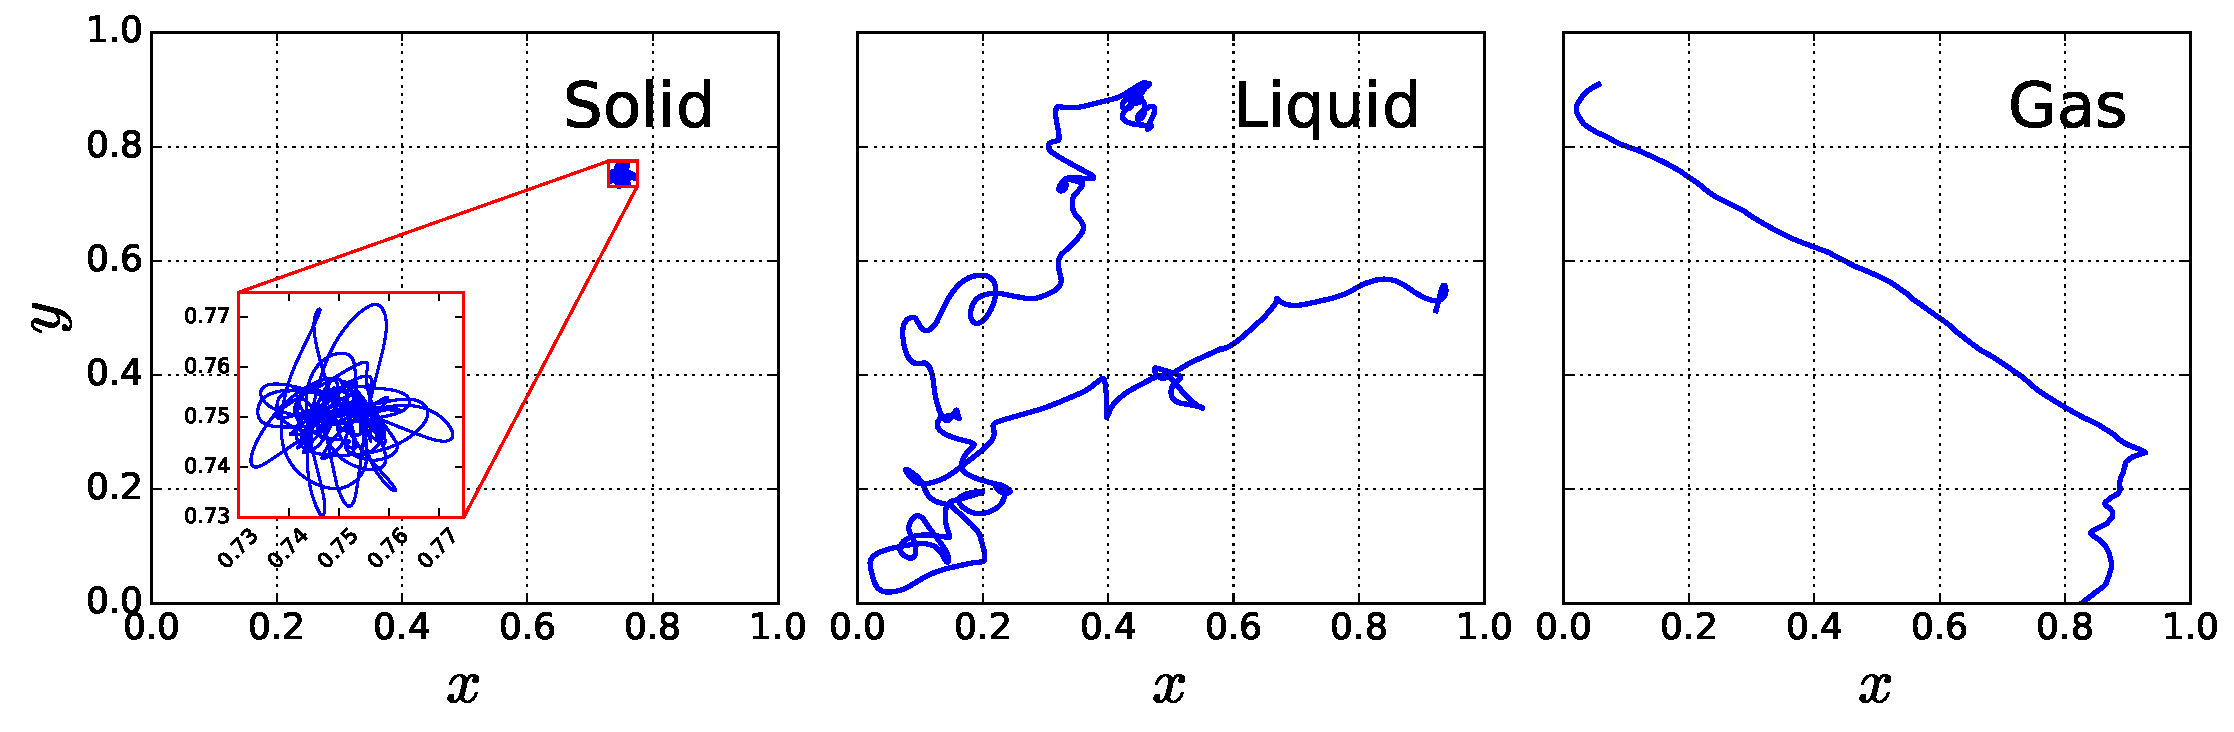
\includegraphics[width=\textwidth]{chapters/ch2-crit/figs/phases}
\end{center}
\caption{How a system of particles behave in the three phases of matter. Here a
    simulation of 100 particles was done, but the trajectory of only one is
    shown. In the solid state the particles are confined to small region by
    the interactions of its neighbors. In the liquid state the particle is
    unconfined, but still interacts strongly with the other particles. In the
    gas state the kinetic energy of the particles is large enough that they
    barely interact with one another, making a ballistic trajectory until
    they make a head-on collision with another particle.}
\label{fig:phases}
\end{figure}

Not all systems have phases related with the states of matter, however. Some
are related to magnetic or electric properties. This is the case of
ferromagnetic materials, materials that exhibit a persistent magnetization
after being subject to a strong magnetic field, like your everyday fridge
magnet. This phenomenon is a result of the alignment of the magnetic spins of
the atoms or molecules that compose the material. In contrast, paramagnetic
materials show no permanent magnetization. If you take a magnet and raise its
temperature, eventually the thermal fluctuations will misalign the spins,
zeroing out the magnetization and turning the ferromagnetic material into a
paramagnetic one. Other examples of phase transitions also include the
transition of a material into a superconductive state~\cite{Fisher1991} or when
helium turns into into a superfluid~\cite{Campostrini2006}, both happening at
very low temperatures.

To better visualize the different phases of systems, it is common to make use
of a \textit{phase diagram}. Simply put, a phase diagram is a graph where each
axis represent one control parameter, and every point in this graph is labeled
according to the phase the system finds itself for that value of the
parameters. Figure~\ref{fig:water}a shows the very famous phase diagram of
water as a function of temperature and pressure. The three main phases (solid,
liquid and gas) are clearly marked, and the black lines are the boundary
between the phases. Crossing any of these lines is followed by a sharp change
on the properties of the system, as described previously. This is know as a
\textit{phase transition}.

\begin{figure}[t]
\begin{center}
    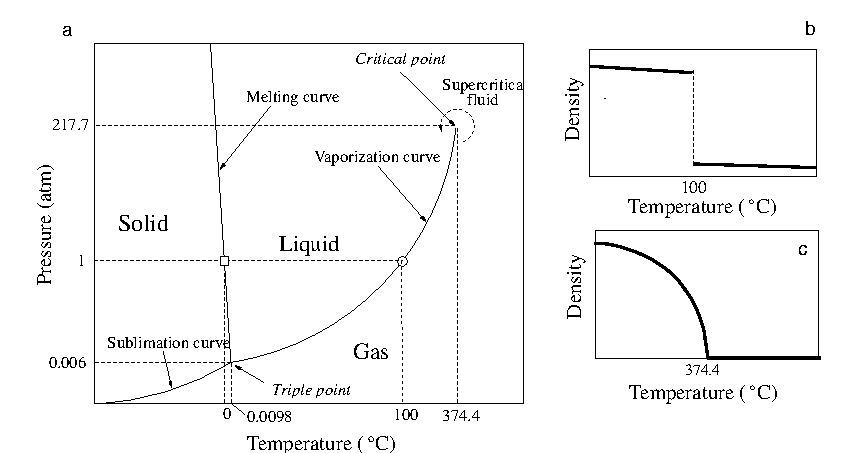
\includegraphics[width=0.8\textwidth]{chapters/ch2-crit/figs/water}
\end{center}
\caption{Phase diagram of water (a). Here, the three usual phases are
    distinguished, each separated from the other by a coexistence line. The
    phase transition that happens when the system traverse a line is
    characterized by a discontinuous jump in the density, as shown in (b) for
    the liquid-gas transition at $P=1$ atm. For $P=217.7$ atm however the same
    transition is continuous, as shown in (c). In the vicinity of this phase
    transition, at $T\approx374.4^\circ$C, the two phases become
    indistinguishable, and display a number of peculiarities. Systems in such
    state are called critical systems. Reproduced from~\cite{Sole2011}.}
\label{fig:water}
\end{figure}


\section{Classification of Phase Transitions}
\label{sec:classification}

Phase transitions are usually classified into two categories: first and second
order. There is no consensus on the precise definition of each, but this does
not matter a lot, since they behave quite differently. An old, but still often
used definition was proposed by Ehrenfest~\cite{Jaeger1998}. But, before we get
into that, we have to find a quantitative way of describing the phase of a
system. This is done by defining an \textit{order parameter}, a quantity that
take very distinct values in different phases (usually normalized to be zero in
the most disordered phase). In the case of water, the order parameter is the
density (which is just the inverse of the volume). For ferromagnetic
transitions we use the spontaneous magnetization. The choice of order parameter
for several systems can be seen in Table~\ref{tab:ptex}.

\begin{table}
\newcolumntype{L}[1]{>{\raggedright\let\newline\\\arraybackslash\hspace{0pt}}m{#1}}
\begin{centering}
\begin{tabular}{L{4cm}L{5cm}L{2cm}L{2.0cm}L{0mm}}
\bottomrule[0.1mm]
\toprule[0.1mm]
\textbf{Transition Type}   & \textbf{Order Parameter}                         & \textbf{Example}          & $\mathbf{T_{c}}$ \textbf{(K)}   &\\
\bottomrule[0.1mm]
Liquid-gas                 & Molar volume                                     & H$_{2}$O                  & 647.05~\cite{Leveltsengers1974} &\\[0.5cm]
Ferromagnetic              & Magnetic moment                                  & Fe                        & 1044.0~\cite{Kadanoff1967}      &\\[0.5cm]
Antiferromagnetic          & Sublattice magnetic moment                       & FeF$_{2}$                 & 78.26~\cite{Ahlers1974}         &\\[0.5cm]
$\lambda$-line in $^{4}$He & $^{4}$He quantum mechanical amplitude            & $^{4}$He                  & 1.7--2.1~\cite{Ahlers1973}      &\\[0.5cm]
Superdonductivity          & Electron pair amplitude                          & Pb                        & 7.19~\cite{Heller1967}          &\\[0.5cm]
Binary fluid mixture       & Fractional segregation of components             & CCl$_{4}$-C$_{7}$F$_{14}$ & 301.78~\cite{Heller1967}        &\\[0.5cm]
Binary alloy               & Fraction of one atomic species on one sublattice & Cu-Zn                     & 739~\cite{Dietrich1966}         &\\[0.5cm]
Ferroelectric              & Electric dipole moment                           & Triglycine sulfate        & 322.5~\cite{Gonzalo1966}        &\\[0.5cm]
\bottomrule[0.1mm]
\toprule[0.1mm]
\end{tabular}
\par\end{centering}
\caption{Examples of systems that display a second order phase transition.
    Reproduced from~\cite{Shang2000}.}
\label{tab:ptex}
\end{table}


Following the example of water, where the temperature and pressure are the
control variables, the thermodynamic properties are determined by the Gibbs
free energy
\begin{equation}
    G=E-TS+pV.
\end{equation}
from which we can obtain the volume by taking its derivative
\begin{equation}
    V={\left(\frac{\partial G}{\partial p}\right)}_T.
\end{equation}
If we now make an experimental apparatus to try and observe how the density of
an amount of water behaves during a phase transition, say the liquid-gas
transition, what we see is shown in Figure~\ref{fig:water}b. The density (and
therefore the volume) makes a discontinuous jump.

This transition is characterized by the presence of latent heat, an amount of
energy that the system releases or absorbs during a phase transition, which is
a constant of the substance, and is independent on the temperature, pressure or
other control parameters~\cite{Callen1985}. This means that when boiling a
volume of water, the temperature of the liquid phase does not rise because the
extra heat being added is being absorbed in form of latent heat. Because you
add disorder to the system without changing its temperature, it happens that
the entropy, another derivative of $G$,
\begin{equation}
    S=-{\left(\frac{\partial G}{\partial T}\right)}_p,
\end{equation}
is also discontinuous at the boundary of a phase transition. Because the first
derivatives of the free energy display a discontinuity, we say these phase
transitions are of \textit{first order}. This sudden change happens because the
equilibrium state of the system (determined by the minimum of the free energy)
shifts from one part of the phase space to another~\cite{Callen1985}, as
illustrated in Figure~\ref{fig:gibbs1}. When the system is exactly at the
boundary of the phase transition, the two phases have the same free energy,
allowing them both to coexist in different regions of the system. Because of
this, the transition lines are also called coexistence lines. On the point
labeled triple point, the free energy has \textit{three} equal minima, so all
three phases (solid, liquid and gas) exist on the same system. Because the
triple point is uniquely defined, it is the basis used to define the Kelvin
temperature scale~\cite{Fermi1956}.

\begin{figure}[t]
\begin{center}
    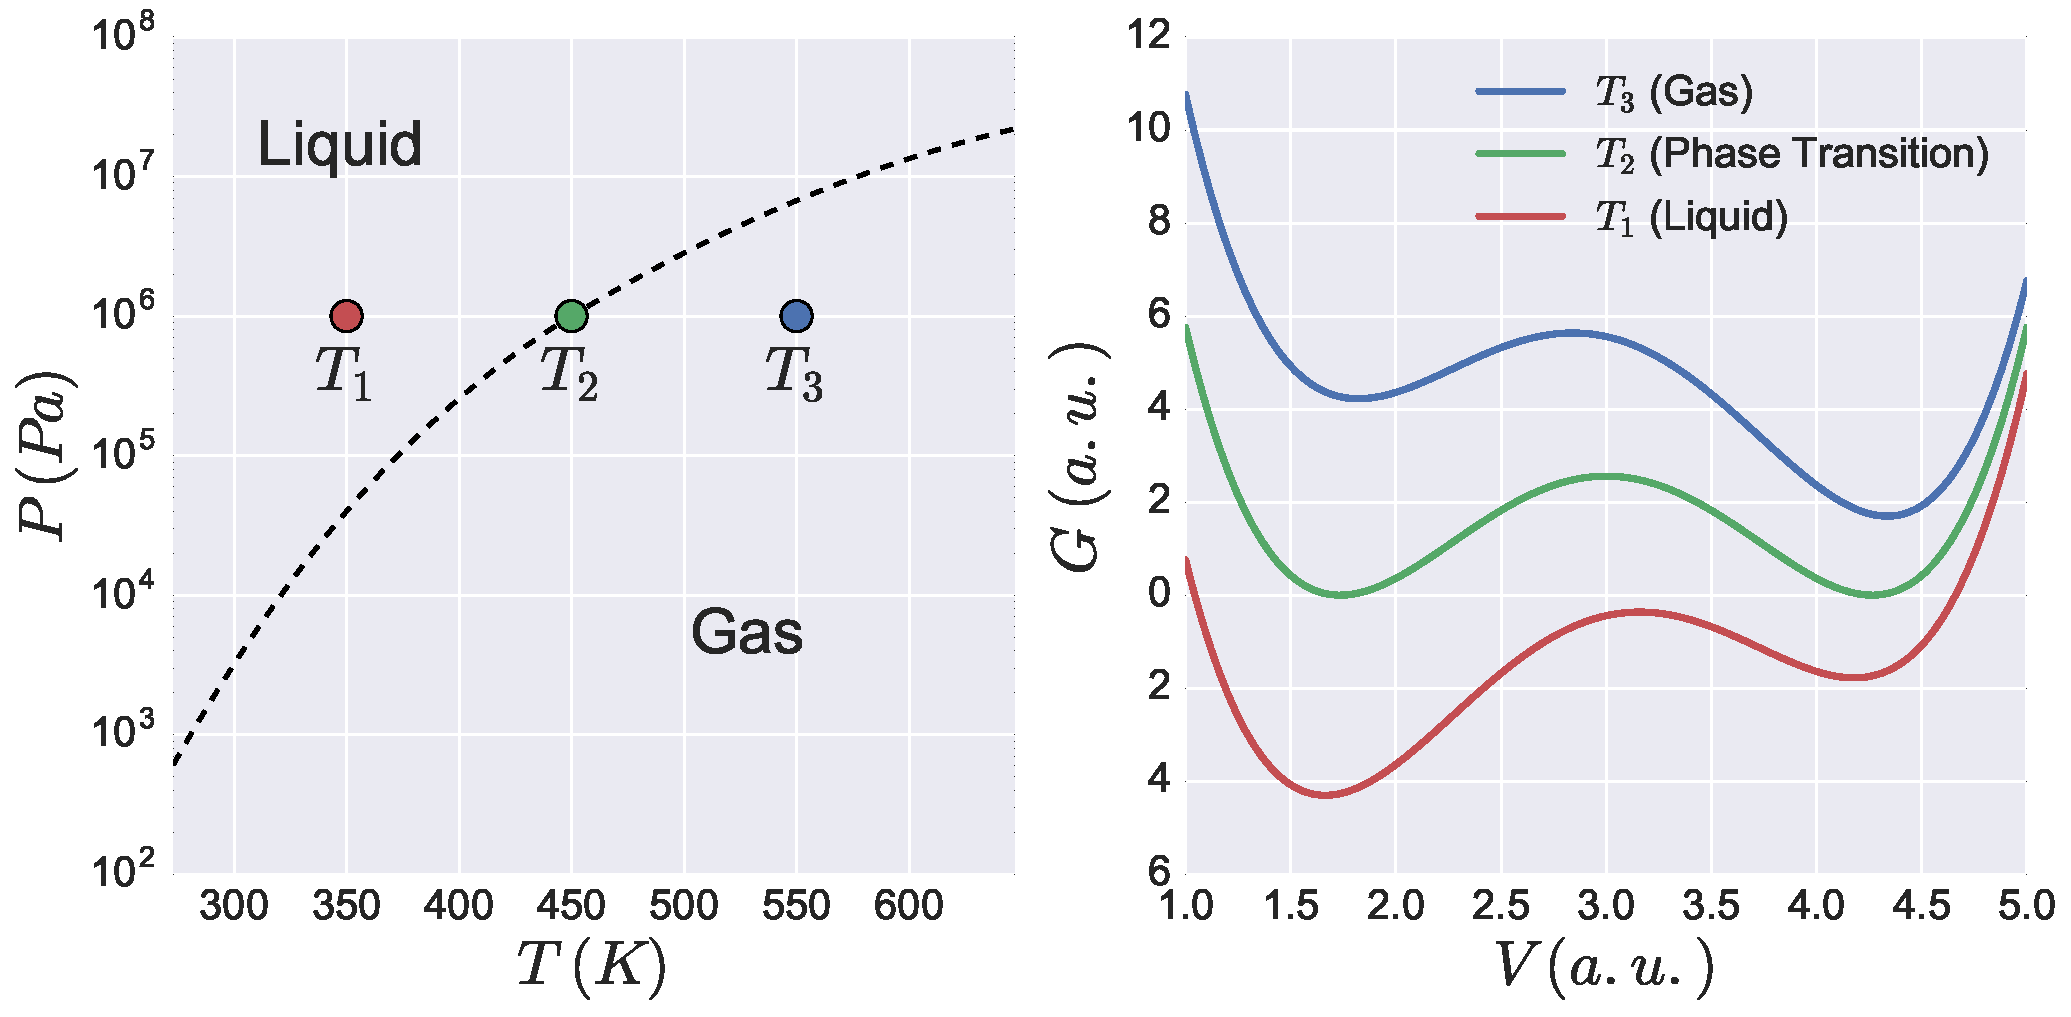
\includegraphics[width=0.8\textwidth]{chapters/ch2-crit/figs/gibbs1}
\end{center}
\caption{Why first order transitions happen. The left graph shows three points
    on the phase space of water. The red one is in the liquid phase, the blue
    is in the gaseous state and the green right on the boundary. The right
    graph shows a heuristic construction of the Gibbs free energy in each of
    the three points (matched by color). The equilibrium state is the one of
    minimal free energy. Although $G$ changes continuously with the
    temperature, the global minimum shifts abruptly once the phase boundary is
    crossed, thus occurring a first order phase transition. When the system is
    exactly on the boundary, the minima are equivalent, and the two phases
    coexist.}
\label{fig:gibbs1}
\end{figure}

Now, looking again at Figure~\ref{fig:water}a one might ask why the liquid-gas
transition line does not extend all the way through the phase diagram. This
is where things start to get interesting. We have established that the free
energy have two equivalent minima when the system is over the coexistence line.
Now, if we walk along this line following the behavior of the free energy, what
we observe is that the ``dividing barrier'' between  the two minima gets shorter
and shorter, similar to what is shown in Figure~\ref{fig:gibbs2}. At a critical
temperature of approximately $374^\circ$C and pressure of $217.7$atm, the two
minima merge. At this point it is not that the two phases coexist, they are
indistinguishable from one another.

If we look at the order parameter when the system pass through the critical
point, we see that it is no longer discontinuous, as it is shown in
Figure~\ref{fig:water}c. If we set the pressure to the same as the critical
point and heat an amount of liquid water, the volume will rise continuously
(although not necessarily smoothly) until it reaches the gaseous state. Not all
quantities are well behaved though. The ones that do display discontinuities on
the critical point, are the second derivatives of the free energy, like the
specific heat
\begin{equation}
    c_p=T{\left(\frac{\partial S}{\partial T}\right)}_{p}=
    T{\left(\frac{\partial^{2}G}{\partial T^{2}}\right)}_{p},
\end{equation}
or the isothermal compressibility
\begin{equation}
    \kappa_T=-\frac{1}{V}{\left(\frac{\partial V}{\partial p}\right)}_{T}=
    -\frac{1}{V}{\left(\frac{\partial^{2}G}{\partial p^{2}}\right)}_{T}.
\end{equation}
Figure~\ref{fig:suscep} shows two examples of such discontinuities in real
system. Because the second derivative of the free energy is discontinuous,
going through a critical point is know as a \textit{second order} phase
transition, and systems close to it are called \textit{critical systems}.

Second order transitions have a whole range of peculiar behavior associated
with it. The most notorious is the presence of large fluctuations. In
Chapter~\ref{ch:intr} we mentioned the work of Thomas
Andrews~\cite{Andrews1869}, who noticed that some substances become opaque at
the critical point. This happens because the huge fluctuations in the spacial
distribution of mass, forming water ``droplets'' of all sizes, including the
sizes that scatter most visible light, giving the system a milky aspect.

Although we focused a lot on the example of water, the ferromagnetic transition
described in the previous section is probably the most studied kind of second
order phase transition. Its free energy is given by
\begin{equation}
    dF = -SdT-Mdh
\end{equation}
where $M$ is the spontaneous magnetization (the order parameter in this case)
and $h$ is an uniform external magnetic field. It is characterized by a
diverging magnetic susceptibility
\begin{equation}
    \chi_{M}=
    {\left(\frac{\partial M}{\partial h}\right)}_{T}=
    -{\left(\frac{\partial^{2}F}{\partial h^{2}}\right)}_{T}.
\end{equation}

\begin{figure}
\begin{center}
    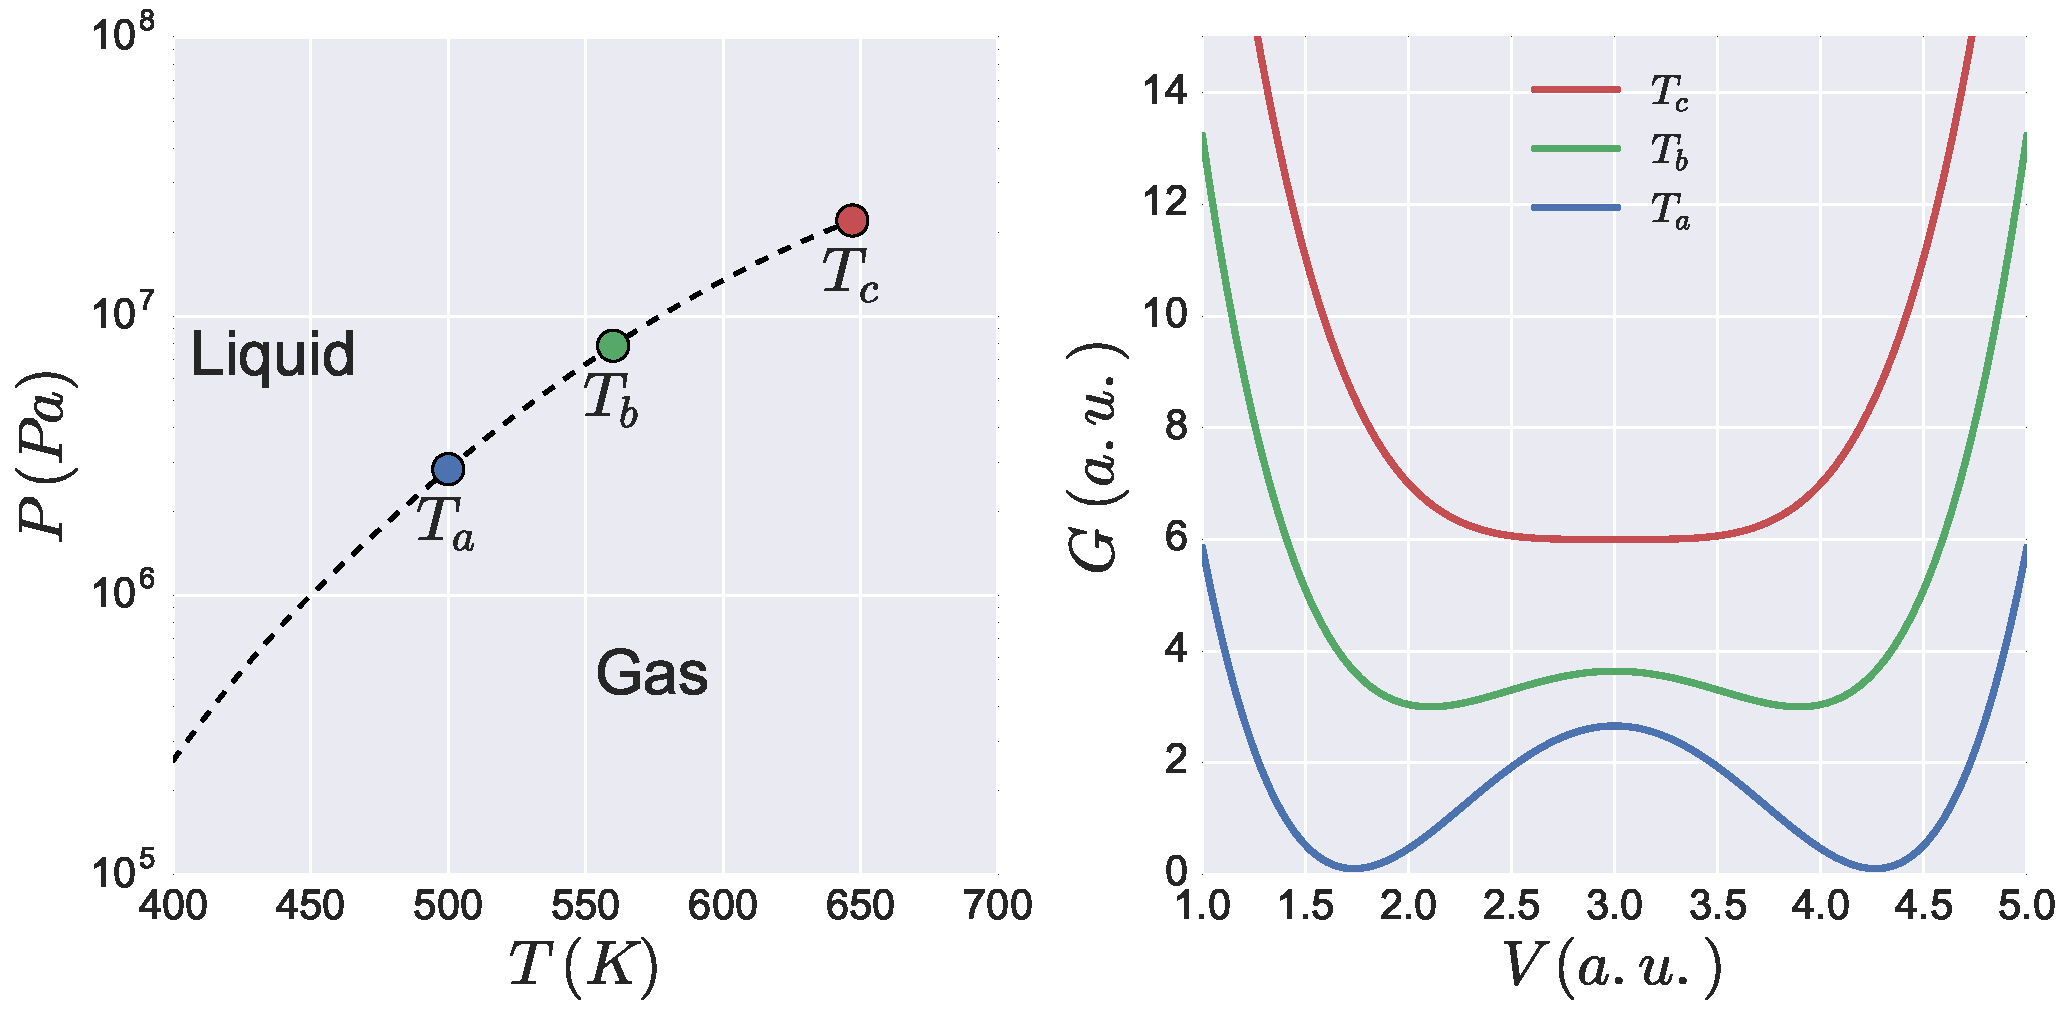
\includegraphics[width=0.8\textwidth]{chapters/ch2-crit/figs/gibbs2}
\end{center}
\caption{If we follow the (heuristic) Gibbs free energy along the liquid-gas
    line, we observe that at some critical point $T_c$ the two minima (related
    to the liquid and gas phases) coalesce into one. At this point the two
    phases are indistinguishable, which characterizes a second order phase
    transition. Systems close to the critical point are called critical
    systems.}
\label{fig:gibbs2}
\end{figure}


\begin{figure}
\begin{center}
    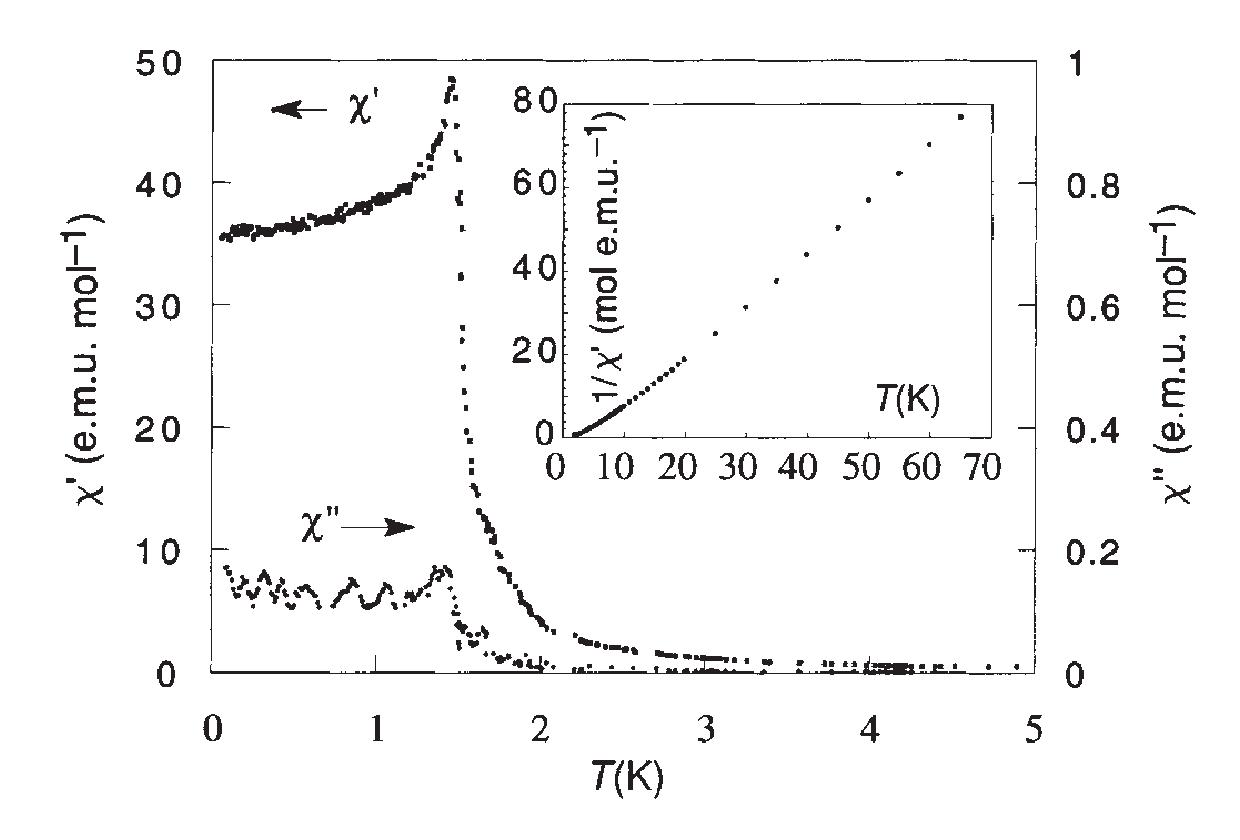
\includegraphics[width=1.0\textwidth]{chapters/ch2-crit/figs/suscep}
\end{center}
\caption{Examples of thermodynamical quantities in the vicinity of a second
    order phase transitions. The left graph shows the diverging magnetic
    susceptibility on the ferromagnetic transition of
    dupeyredioxyl~\cite{Chiarelli1993}. The graph on the right shows the
    diverging specific heat of the lambda transition of superfluid
    helium-4~\cite{Keesom1935}.}
\label{fig:suscep}
\end{figure}

Not all phase transitions fall neatly into these two categories, however. The
Kosterlitz-Thouless transition of the XY-Model (related to some superconducting
transitions~\cite{Resnick1981}) could be considered of infinite order, because
the free energy is infinitely differentiable~\cite{Kosterlitz1973}, although it
shares some similarities with second order transitions.

The discussion of phase transitions presented so far, rooted on the postulates
of thermodynamics and in the analyticity of the free energy, is due to
Landau~\cite{Landau1969}. While this theory manages to capture a few properties
of critical systems, it fails catastrophically from a quantitative standpoint.
The source of this discrepancy comes from some basic assumptions of statistical
mechanics. You see, the maximum entropy postulate is derived from the fact that
the probability of finding a system in any given state is distributed very
narrowly around a value, this way we can assume the expected (average) energy
of the system is the same as the most probable one. On the critical point
however, because the minimum of the free energy is so shallow, the probability
distribution broadens significantly, so much that the difference between most
probable and average cannot be ignored~\cite{Callen1985}.


\section{Critical Exponents and Universality}
\label{sec:universality}
\newcommand{\op}{\phi}
\newcommand{\sfi}{J}

We noted that several thermodynamical quantities diverge on the critical point.
More important than that is to know \textit{how} they diverge. This motivates
the definition of a set of indices called \textit{critical exponents} that
characterize the behavior of the system near the critical point. Here we will
use $\op$ for the order parameter (the density for water, the magnetization for
ferromagnets) and $\sfi$ for the source field (pressure for water, the external
magnetic field for ferromagnets). This way we can define a generalized
susceptibility $\chi=\partial\op/\partial \sfi$ and specific heat
$c=-\partial^2 f / \partial T^2$.

In the thermodynamics domain there are four main critical exponents, each
associated with a different quantity. We have the heat capacity exponent
$\alpha$
\begin{equation}
    \label{eq:heatc}
    \begin{array}{ccccc}
        c & \sim & {\left(T-T_c\right)}^{-\alpha}  & \mbox{for} & T > T_c \\
        c & \sim & {\left(T_c-T\right)}^{-\alpha'} & \mbox{for} & T < T_c,
    \end{array}
\end{equation}
the order parameter exponent $\beta$, when taken along the coexistence curve 
\begin{equation}
    \begin{array}{ccccc}
        \op  & \sim & {\left(T_c-T\right)}^{\beta} & \mbox{for} & T < T_c,
    \end{array}
\end{equation}
the generalized susceptibility exponent $\gamma$
\begin{equation}
    \begin{array}{ccccc}
        \chi  & \sim & {\left(T-T_c\right)}^{-\gamma}  & \mbox{for} & T > T_c \\
        \chi  & \sim & {\left(T_c-T\right)}^{-\gamma'} & \mbox{for} & T < T_c,
    \end{array}
\end{equation}
and the order parameter exponent $\delta$, when taken at constant temperature
$T=T_c$
\begin{equation}
    \begin{array}{ccccc}
        \op  & \sim & {\left(\sfi-\sfi_c\right)}^{1/\delta} & \mbox{for} & \sfi > \sfi_c.
    \end{array}
\end{equation}
These exponents may have different values if you take the limit from above or
bellow the critical point (unprimed and primed symbols respectively), but
unless explicitly noted, we will assume that they are the same, which happens
often.

There are many other critical exponents outside the realm of thermodynamics.
These exponents can only be studied by a full statistical mechanical framework.
Two of the most important ones are related to the correlations of the system.
Take the ferromagnetic transition, for instance. The influence of an individual
spin is usually restricted over a finite region around it. That is to say,
there is a length scale $\xi$ that if we take two spins separated by a distance
$r\ll\xi$ and flip one of the spins, the other is very likely to also flip. In
the unordered (paramagnetic) phase, $\xi$ is small because the thermal
fluctuations inhibit long range correlations. On the ordered (ferromagnetic)
phase, the influence of large clusters of aligned spins is stronger than that
of a single one, also hindering the range of correlations. We see that too
much order, as well as too much disorder, have the effect of restricting the
influence of the spins over each another. Therefore, it makes sense to think
that somewhere in between there is a sweet spot where the balance between order
and disorder makes the correlation length as large as possible.

We can formalize this thought by defining the correlation function of a system
\begin{equation}
    \label{eq:corr0}
    C_{\op}\left(\left|\mathbf{r_1}-\mathbf{r_2}\right|\right) = 
    \left\langle
        \op\left(\mathbf{r_{1}}\right)
        \op\left(\mathbf{r_{2}}\right)
    \right\rangle -
    \left\langle
        \op\left(\mathbf{r_{1}}\right)
    \right\rangle
    \left\langle
        \op\left(\mathbf{r_{2}}\right)
    \right\rangle
\end{equation}
where $\op\left(\mathbf{r}\right)$ is the local value of the order parameter at
any given point of the system. The macroscopic value can be recovered from its
expected value $\op=V^{-1}\int\op(x)d^d x$. The assumption that
$C\left(\mathbf{r_1},\mathbf{r_{2}}\right) =
C\left(\left|\mathbf{r_{1}}-\mathbf{r_{2}}\right|\right)$ comes from
translation invariance, which takes no specific point of the system as special.
It is natural to expect that the correlations would decay exponentially, with a
decay constant $\xi$
\begin{equation}
    \label{eq:corr}
    C\left(r\right)\sim e^{-r/\xi}.
\end{equation}

The relation between thermodynamics and the correlation function is governed
by the fluctuation-dissipation theorem~\cite{Henkel2013}
\begin{equation}
    \label{eq:flucdiss}
    \chi=\frac{\partial\op}{\partial \sfi}=\frac{1}{T}\int C\left(r\right)dr.
\end{equation}
We know that on the critical point $\chi$ diverges, but  the integral on the
right-hand side cannot diverge for finite $\xi$, given Eq.~\ref{eq:corr}.
The conclusion is simple, not only the correlation length is maximal at the
critical point, it is infinite! This divergence also has a critical exponent
$\nu$ associated with it
\begin{equation}
    \label{eq:corlen}
    \begin{array}{ccccc}
        \xi & \sim & {\left(T-T_c\right)}^{-\nu}  & \mbox{for} & T > T_c \\
        \xi & \sim & {\left(T_c-T\right)}^{-\nu'} & \mbox{for} & T < T_c.
    \end{array}
\end{equation}
At the critical point, the correlation function itself also cannot decay as an
exponential, and goes instead as a power law, with yet another critical
exponent $\eta$
\begin{equation}
    \label{eq:critcor}
    \begin{array}{ccccc}
        C(r) & \sim & r^{-d+2-\eta} & \mbox{for} & T = T_c.
    \end{array}
\end{equation}
where $d$ is the number of spatial dimensions (usually 2 or 3, but it is often
useful to leave it as a variable parameter~\cite{Wilson1972}). 
%This is no minor
%fact, it means that near the critical point, all length scales contribute to
%the overall behavior of the system, making it that much more complicated to
%treat. Unlike, say, in fluid dynamics, where you do not need to know the details
%about the intermolecular interaction of water molecules to predict the ocean
%tides, in critical systems the large and small length scales are indissociable.
Many authors consider this fact, that very distant particles can influence the
state of each other, to be the defining characteristic of a second order phase
transition.

\begin{table}
\newcolumntype{L}[1]{>{\raggedright\let\newline\\\arraybackslash\hspace{0pt}}m{#1}}
\begin{centering}
\begin{tabular}{r>{\raggedright}m{2.6cm}L{1.3cm}L{1.2cm}L{1.2cm}L{1.1cm}L{1.1cm}L{1.0cm}}
\bottomrule[0.1mm]
\toprule[0.1mm]
\textbf{Class}     & \textbf{Examples}   & \boldmath$\alpha$ & \boldmath$\beta$ & \boldmath$\gamma$ & \boldmath$\delta$ & \boldmath$\nu$ & \boldmath$\eta$  \\
\bottomrule[0.1mm]
Mean Field         & ---                 & $0$               & $1/2$            & $1$               & $3$               & $1/2$          & $0$     \\[0.5cm]
2D Ising           & Ferromagnet         & $0$               & $1/8$            & $7/4$             & $15$              & $1$            & $1/4$   \\[0.5cm]
3D Ising           & Liquid-Vapor        & $0.11$            & $0.33$           & $1.24$            & $4.79$            & $0.63$         & $0.036$ \\[0.5cm]
3D XY-Model        & Superfluid $^{4}$He & $-0.015$          & $0.348$          & $1.31$            & $4.78$            & $0.671$        & $0.038$ \\[0.5cm]
2D 3-State Potts   & Cubic ferromagnet   & $1/3$             & $1/9$            & $13/9$            & $14$              & $5/6$          & $4/15$  \\[0.5cm]
2D Percolation     & Porous Media        & $-2/3$            & $5/36$           & $43/18$           & $91/5$            & $4/3$          & $5/24$  \\[0.5cm]
\bottomrule[0.1mm]
\toprule[0.1mm]
\end{tabular}
\par\end{centering}
\caption{Non exaustive list of critical exponents of various universlity
    classes~\cite{Callen1985, Onsager1944, ElShowk2014, Guillou1977, Wu1982,
    Smirnov2001}. Thke mean field is the result found using the Landau approach
    shown in Section~\ref{sec:classification}, it is an approximation of high
    dimensional systems.}
\label{tab:univ}
\end{table}


The most notable consequence of the dominance of long range correlations is
that the critical behavior of the system is determined by the general
properties of the fluctuations, which in turn are mainly determined by the
dimensionality of the system and of the order parameter, and not by the details
of the material that compose the system~\cite{Stanley1999}. As a consequence,
all systems tend to group themselves into classes that share the same critical
exponents. These are called \textit{universality classes}. For example, the
liquid-gas transition falls in the same universality class as the ferromagnetic
transition~\cite{Kim1984}. Table~\ref{tab:univ} show some examples of
universality classes, systems that belong to it, and the values of their
critical exponents.


\section{Scaling Invariance}
\label{sec:scalinginv}
\renewcommand{\op}{\phi}

The list of critical exponents shown on the last section is far from
exhaustive. More exotic, but no less important exponents include the fractal
dimension~\cite{Voss1984}, one-arm exponent~\cite{Lawler2001b} and the crossing
exponent~\cite{Aizenman1999}, among others. It sure seems like a lot of work to
completely describe a universality class, if one needs to compute dozens of
exponents. Luckily with the very simple assumption of scaling invariance, we
can greatly reduce the amount of work needed.

We will take a look at the correlation functions of the observables, which
we will refer as \textit{scaling operators}. The main ones are the order
parameter distribution $\op(\mathbf{r})$ and energy density
$\varepsilon(\mathbf{r})$. The two-point correlation function of these fields is
defined according to Eq.~\ref{eq:corr0}
\begin{eqnarray}
    \label{eq:corr10}
    C_{\op}\left(\left|\mathbf{r_1}-\mathbf{r_2}\right|\right) & = &
    \left\langle
        \op\left(\mathbf{r_{1}}\right)
        \op\left(\mathbf{r_{2}}\right)
    \right\rangle -
    \left\langle
        \op\left(\mathbf{r_{1}}\right)
    \right\rangle
    \left\langle
        \op\left(\mathbf{r_{2}}\right)
    \right\rangle,
    \\
    \label{eq:corr11}
    C_{\varepsilon}\left(\left|\mathbf{r_1}-\mathbf{r_2}\right|\right) & = &
    \left\langle
        \varepsilon\left(\mathbf{r_{1}}\right)
        \varepsilon\left(\mathbf{r_{2}}\right)
    \right\rangle-
    \left\langle
        \varepsilon\left(\mathbf{r_{1}}\right)
    \right\rangle
    \left\langle
        \varepsilon\left(\mathbf{r_{2}}\right)
    \right\rangle.
\end{eqnarray}
They are given in terms of the reduced temperature and source field
\begin{equation}
    t=\frac{T-T_c}{T_c},\;\;\;\;\;\;\;\;\;h=\frac{\sfi-\sfi_c}{\sfi_c},
\end{equation}
so the critical point is exactly at $t=0$ and $h=0$. These are also known
as \textit{scaling fields}.

The scaling hypothesis postulates that the correlation functions transform
under a scaling transformation $\mathbf{r}\rightarrow\mathbf{r}/b$ in the
following way
\begin{eqnarray}
    \label{eq:scal}
    C_{\op}\left(\mathbf{r};t,h\right) & = &
    b^{-2x_{\op}}C_{\op}\left(\mathbf{r}/b;tb^{y_{t}},hb^{y_{h}}\right)\\
    \label{eq:scal10}
    C_{\varepsilon}\left(\mathbf{r};t,h\right) & = &
    b^{-2x_{\varepsilon}}C_{\varepsilon}\left(\mathbf{r}/b;tb^{y_{t}},hb^{y_{h}}\right)
\end{eqnarray}
where $x_\op$ and $x_\varepsilon$ are the \textit{scaling dimension} of the
scaling operators $\op$ and $\varepsilon$, and $y_t$ and $y_h$ are called the
\textit{renormalization group eigenvalues} of their respective scaling fields.

Following the fluctuation-dissipation theorem, Eq.~\ref{eq:flucdiss}, we can
compute the susceptibility and the specific heat by integrating $C_\op$ and
$C_\varepsilon$ respectively. This give us
\begin{eqnarray}
    \label{eq:chi2}
    \chi\left(t,h\right) & = & b^{d-2x_{\op}}\chi\left(tb^{y_{t}},hb^{y_{h}}\right)\\
    \label{eq:c2}
    c\left(t,h\right) & = & b^{d-2x_{\varepsilon}}c\left(tb^{y_{t}},hb^{y_{h}}\right)
\end{eqnarray}
Recall that $\chi=-\partial^2 f/\partial h^2$ and $c=-\partial^2 f/\partial
t^2$, therefore we can integrate Eq.~\ref{eq:chi2} and~\ref{eq:c2} twice,
obtaining the free energy density $f=F/\mathcal{N}$
\begin{equation}
    f\left(t,h\right)=
    b^{d-2x_{\op}-2y_{h}}f\left(tb^{y_{t}},hb^{y_{h}}\right)=
    b^{d-2x_{\varepsilon}-2y_{t}}f\left(tb^{y_{t}},hb^{y_{h}}\right),
\end{equation}
from which we can deduce that $x_\op+y_h = x_\varepsilon+y_t$. As a matter of
fact, the sum is constant for all pairs of scaling dimension and its conjugate
renormalization group eigenvalue. Since this sum does not depend on the fields
themselves, it is safe to assume they depend on the only other parameter, the
number of spatial dimensions, that is
\begin{equation}
    \label{eq:scald}
    x_\op+y_h = x_\varepsilon+y_t = d
\end{equation}
which leaves us with the neat relation
\begin{equation}
    f\left(t,h\right)=b^{-d}f\left(tb^{y_{t}},hb^{y_{h}}\right).
\end{equation}
It is worth noting that this is not really the free energy of the system. The
actual free energy have a singular and a regular part, the one described so
far is the singular part. Near the critical point, however, only the singular
part makes significant contributions to the behavior of the system, so we can
safely ignore the regular part.

The next step is to make the scaling parameter $b$ a function of the
temperature, in order to get rid of one of the arguments of the free energy.
This can be done by making $b=t^{-1/y_t}$, which yields
\begin{equation}
    f\left(t,h\right)=
    t^{d/y_{t}}f\left(1,ht^{-y_{h}/y_{t}}\right)=
    t^{d/y_{t}}\Psi\left(ht^{-y_{h}/y_{t}}\right),
\end{equation}
where $\Psi$ is known as a scaling function, and it is unique for a given
universality class. We can re-obtain the heat capacity by taking
the second derivative as usual
\begin{equation}
    c=-\left.\frac{\partial^2 f}{\partial t^2}\right|_{h=0}
    \sim \left|t\right|^{d/y_h-2}.
\end{equation}
Which is the expected behavior, and from Eq.~\ref{eq:heatc} we have that
$\alpha=2-d/y_t$. A similar process can be done to derive a similar relation
for all four thermodynamical exponents
\begin{eqnarray}
    \label{eq:scal1}
    \alpha & = & 2-d/y_{t}\\
    \beta  & = & \left(d-y_{h}\right)/y_{t}\\
    \gamma & = & \left(2y_{h}-d\right)/y_{t}\\
    \label{eq:scal2}
    \delta & = & y_{h}/\left(d-y_{h}\right).
\end{eqnarray}
This system of equations can be solved to single out the eigenvalues obtaining
the relations
\begin{eqnarray}
    \alpha+2\beta+\gamma              & = & 2\\
    \alpha+\beta\left(1+\delta\right) & = & 2,
\end{eqnarray}
These are know as \textit{scaling relations}~\cite{Rushbrooke1963,
Griffiths1967}, and are some of the greatest results of the scaling
hypothesis, because if you know the value of two of the thermodynamical
exponents, you get the other two for free.

How about the other two exponents, $\nu$ and $\eta$, related to the
correlations of the order parameter, you might ask. We can also find a simple
relation for them by taking Eq.~\ref{eq:scal} and again making $b=t^{-1/y_t}$
\begin{equation}
    C_{\op}\left(\mathbf{r};t,0\right)=
    t^{2x_{\op}/y_{t}}C_{\op}
    \left(\frac{\mathbf{r}}{{\left(1/t\right)}^{1/y_{t}}};1,0\right).
\end{equation}
We can assume that close to criticality (but not exactly on the critical point)
the correlation function depends only on $r/\xi$, because of
Eq.~\ref{eq:corr}. From this follows that
\begin{equation}
    \xi\sim\left|t\right|^{-1/y_t},
\end{equation}
which, using Eq.~\ref{eq:corlen}, implies that
\begin{equation}
    \label{eq:nuscal}
    \nu=\frac{1}{y_t}.
\end{equation}
Now we can repeat the process by making $b=r$ and $t=0$, which will give us
\begin{equation}
    C_{\op}\left(r;0,0\right)=r^{-2d+2y_{h}}.
\end{equation}
Comparing with Eqs.~\ref{eq:critcor} and~\ref{eq:scald}, gives the relation for
$\eta$
\begin{equation}
    \label{eq:etascal}
    \eta=d-2y_h+2.
\end{equation}
Finally we can find a relation between $\nu$ and $\eta$ using
Eqs.~\ref{eq:scal1}--\ref{eq:scal2},~\ref{eq:nuscal} and~\ref{eq:etascal}.
\begin{eqnarray}
    \label{eq:hs1}
    \gamma & = & \nu\left(2-\eta\right)\\
    \label{eq:hs2}
    \alpha & = & 2-d\nu.
\end{eqnarray}
These are known as \textit{hyperscaling relations}, and amazingly no new
critical exponent is needed to determine them, that is, only two are necessary
to completely describe the critical exponents of a second-order phase
transition, which is very convenient. Sadly the hyperscaling relations are not
as sturdy as the scaling relations and can break down under the presence of
dangerously irrelevant operators~\cite{Nishimori2011}.

The arguments and assumptions used throughout this section were historically
motivated through the study of renormalization group
theory~\cite{Pelissetto2002}, which was an important advancement in critical
phenomena when it was first developed, but it goes well beyond the scope of
this work. However, some authors do prefer to look at scaling invariance
through an axiomatic lens, as it was done here, forming a parallel with the
introduction of conformal invariance (see
Section~\ref{ch:conf})~\cite{Henkel2013}.


\section{Models of Critical Systems}
\label{sec:models}

Beyond the phenomenological approach shown up to this point, another way to
advance the knowledge of statistical physics is through model building, where
we look for simple models capable of providing useful insight into practical
situations. Coming up with a fruitful model however can be a very tiresome and
sometimes arcane task, with a lot of trial and error involved. Over decades of
study, a select group of models have gained a significant status in the canon
of phase transitions. Two that stand out due to their simplicity and historical
significance are the Ising and percolation models.


\subsection{Ising Model}
\label{sec:ising}

Of all phase transition models, Ising's is definitely the most famous, because,
despite its simplicity, it is capable of capturing all of the main features of
ferromagnetic materials near the critical point. I was also the first model
with a second order phase transition to be analytically solved, and because of
that, today it forms the basis of our understanding of phase transitions to
the point that many latter important models, like the $O(n)$ and Potts
models~\cite{Wu1982}, can be traced back to it.

Simply put, the model consists of a set of classical spins $\{s_i\}$, each
taking one of two values: $1$ or $-1$. They are arranged in a lattice and are
allowed to interact with their nearest neighbors. The Hamiltonian of this
system is given by
\begin{equation}
    \mathcal{H}=
    -J\sum_{\left\langle i,j\right\rangle }s_{i}s_{j}
    -h\sum_{i}s_{i},
\end{equation}
Where $\sum_{\left\langle i,j\right\rangle}$ means a summation over all pairs
of nearest neighbors, and $J$ is the interaction coupling parameter. If we
assume $J>0$, then the first term of the Hamiltonian favors the alignment of
the spins, while the second one favors the alignment with an external magnetic
field. See Figure~\ref{fig:ising} for some configurations $\left\{s_i\right\}$
of the Ising model in two dimensions in a square lattice, which according to
statistical mechanics are distributed with the probability
\begin{equation}
    P\left(\left\{ s_{i}\right\} \right)=
    \frac{e^{-\mathcal{H}\left(\left\{ s_{i}\right\} \right)/k_b T}}
         {\sum_{\left\{ s_{j}\right\} }
          e^{-\mathcal{H}\left(\left\{ s_{j}\right\} \right)/k_b T}}.
\end{equation}
We can see that for higher temperatures, more disordered states (which have
higher energy) are more probable.

\begin{figure}[b]
\begin{center}
    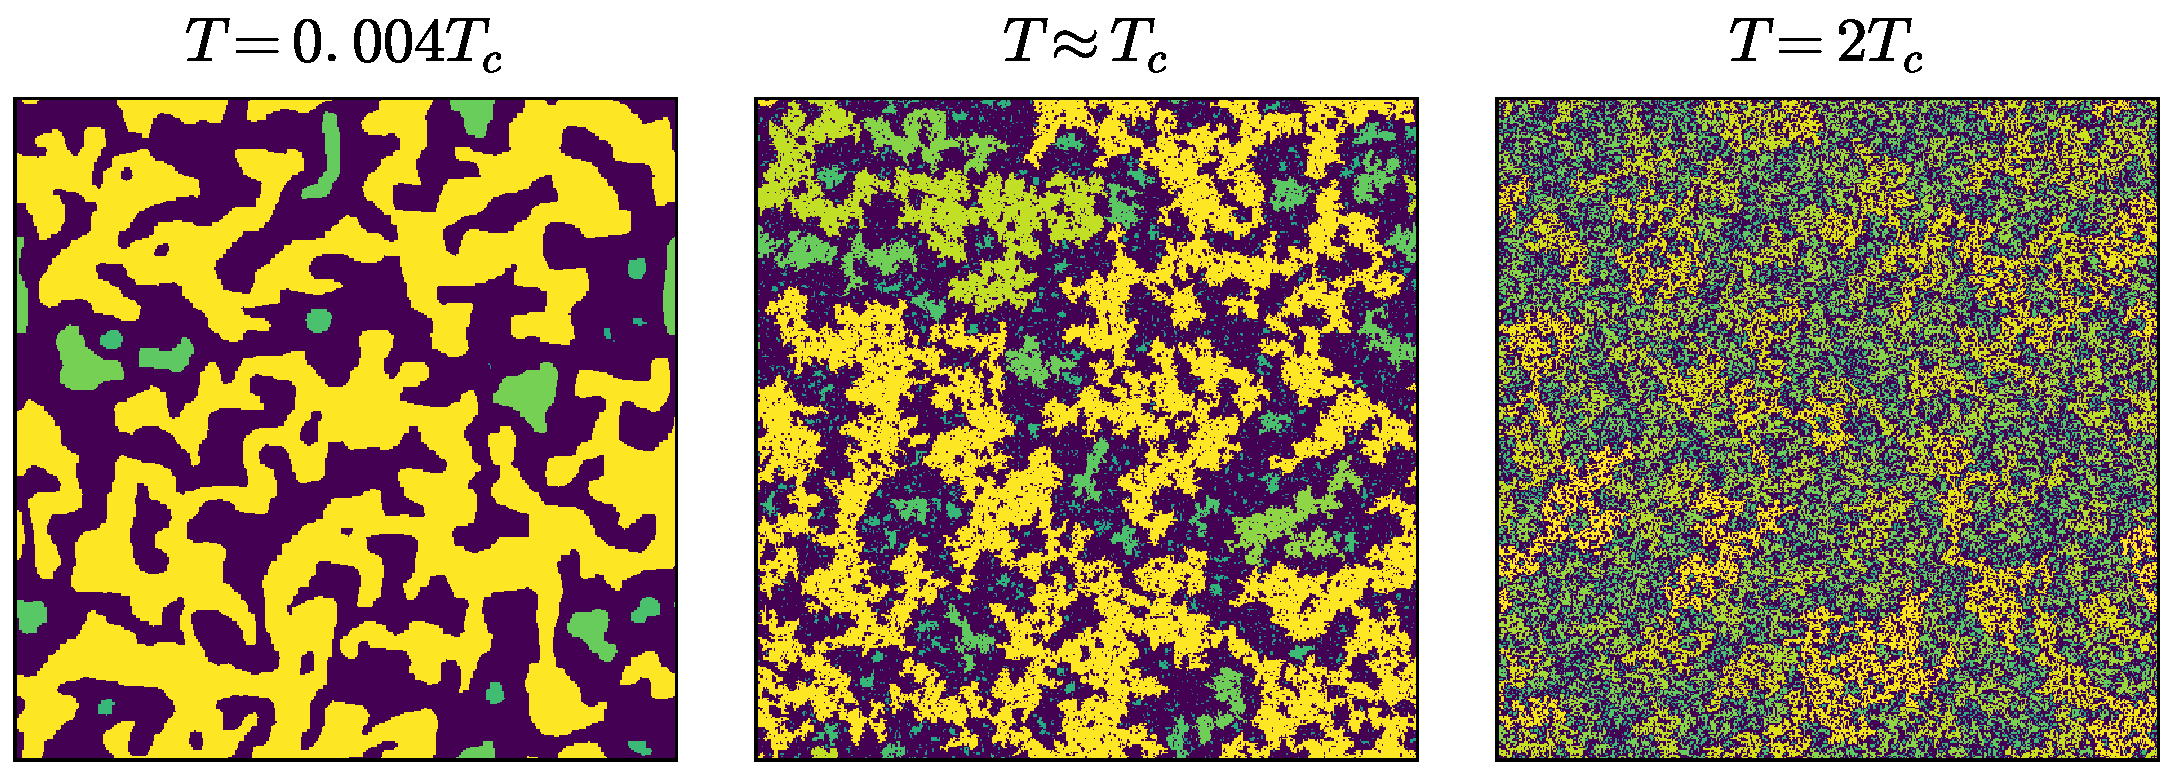
\includegraphics[width=\textwidth]{chapters/ch2-crit/figs/ising}
\end{center}
\caption{Realizations of the Ising model with three different
    temperatures. The clusters of adjacent spin-up sites are colored according
    to how many sites belong to it. The subcritical regime is dominated by the
    large clusters. On the other hand, above the critical point, the system is
    dominated by thermal fluctuations, undermining cluster formation. At the
    critical point however, the clusters lack a characteristic length scale.
    One can observe that the image has a certain ``depth'' to it. This happens
    because clusters of all sizes are present, a mark of scale invariance,
    the most important property of critical systems.}
\label{fig:ising}
\end{figure}


The order parameter here is the spontaneous magnetization $M=\sum_i s_i / N$.
If the temperature is too low the spins will tend to align themselves, giving
rise to an ordered state where $M>0$, while if the temperature is too high,
thermal fluctuations will misalign the spins, resulting in a highly disordered
state with $M=0$.

In his original work~\cite{Ising1925}, Ising solved the model in one dimension,
showing that it does not undergoes a phase transition at finite temperature.
From this result, he mistakenly assumed the same would happen in higher
dimensions. The argument is apparently sound: any configuration of the system
with magnetization $M$ have the same energy as the one where all the spins are
flipped and the magnetization is opposite $-M$. Both configurations have
therefore the same probability $\exp(-E/k_b T)$. The system should then spend
as much time on a positive magnetization as in a negative one, so the average
magnetization should be zero.
On the other hand, Peierls presented an argument for the presence of phase
transitions in $d>1$~\cite{Peierls1936}, showing that in large enough systems
(that is, in the thermodynamic limit) the thermal fluctuations at low
temperatures are not enough to bring the system from a positive magnetization
state to a negative one (and vice-versa), so the system would be ``stuck''
with non-zero magnetization.

\begin{figure}[t]
\begin{center}
    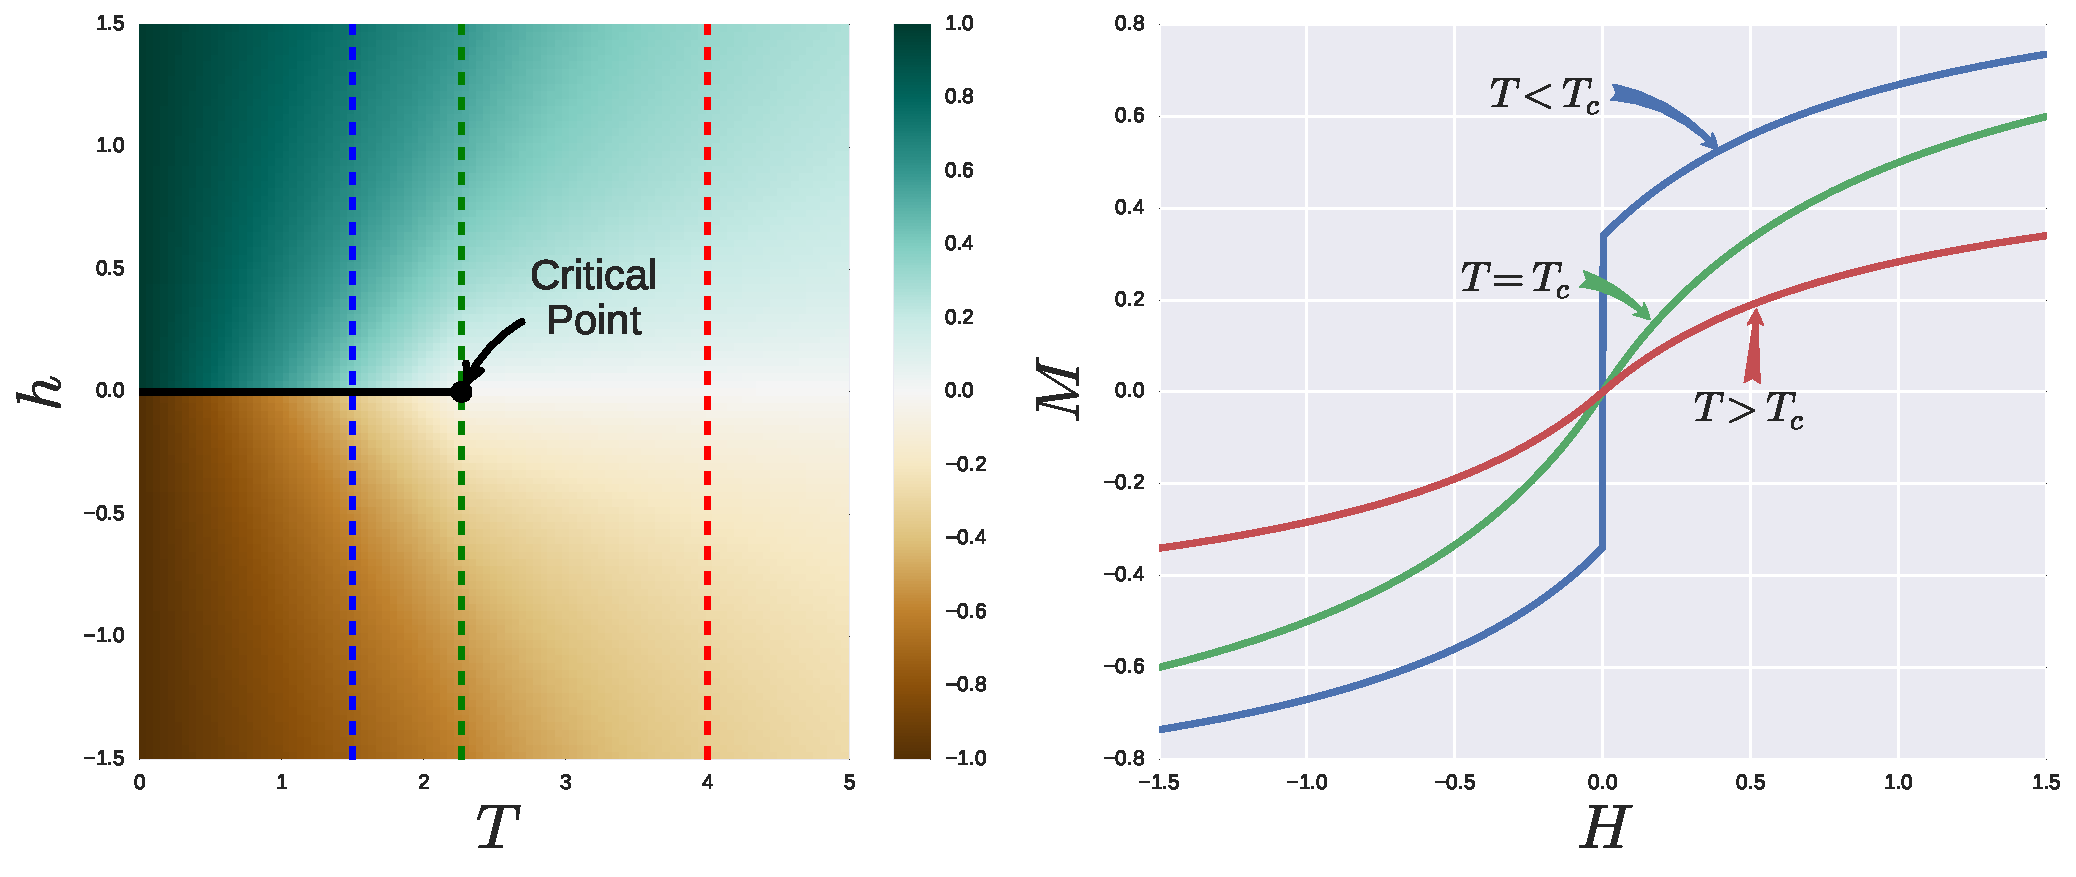
\includegraphics[width=\textwidth]{chapters/ch2-crit/figs/ising_phase2}
\end{center}
\caption{The phase space of the Ising model (left). The color represents the
    spontaneous magnetization $M$ as a function of the external magnetic field
    $h$ and temperature $T$. The black line represents the coexistence line
    where the phase transition is of first order, which means the magnetization
    changes discontinuously like it is shown in the blue line. In the critical
    point (green line), the change becomes continuous and a second order phase
    transition takes place. Beyond this point (red line), the transition is
    always continuous.}
\label{fig:ising_phase2}
\end{figure}

The fact that both of these contradictory arguments seemed correct, led some to
believe that statistical mechanics was inadequate to deal with critical
systems. The solution for this conundrum came from Onsager in
1944~\cite{Onsager1944} who solved the Ising model in a 2D square lattice. The
solution, albeit very complex, demanded no further assumptions than that of
standard statistical physics, a truly remarkable and well celebrated result.
The mistake in Ising's argument lies on the partition function,
\begin{equation}
    \mathcal{Z}=
    \sum_{\left\{ s_{i}\right\} }
    \exp\left[
        -\frac{\mathcal{H}\left(\left\{ s_{i}\right\} \right)}{k_{b}T}
    \right],
\end{equation}
from which follow all thermodynamic properties~\cite{Pathria1996}. The
partition function is certainly analytical in $T$ for a finite system, because
the number of different configurations $\{s_i\}$ is finite, and a finite sum of
exponentials is an analytical function. However, if the number of
configurations is infinite, which should happen in the thermodynamic limit, the
analyticity cannot be guaranteed, and the singularities typical of a second
order phase transition are allowed to come about.

\begin{figure}[t]
\begin{center}
    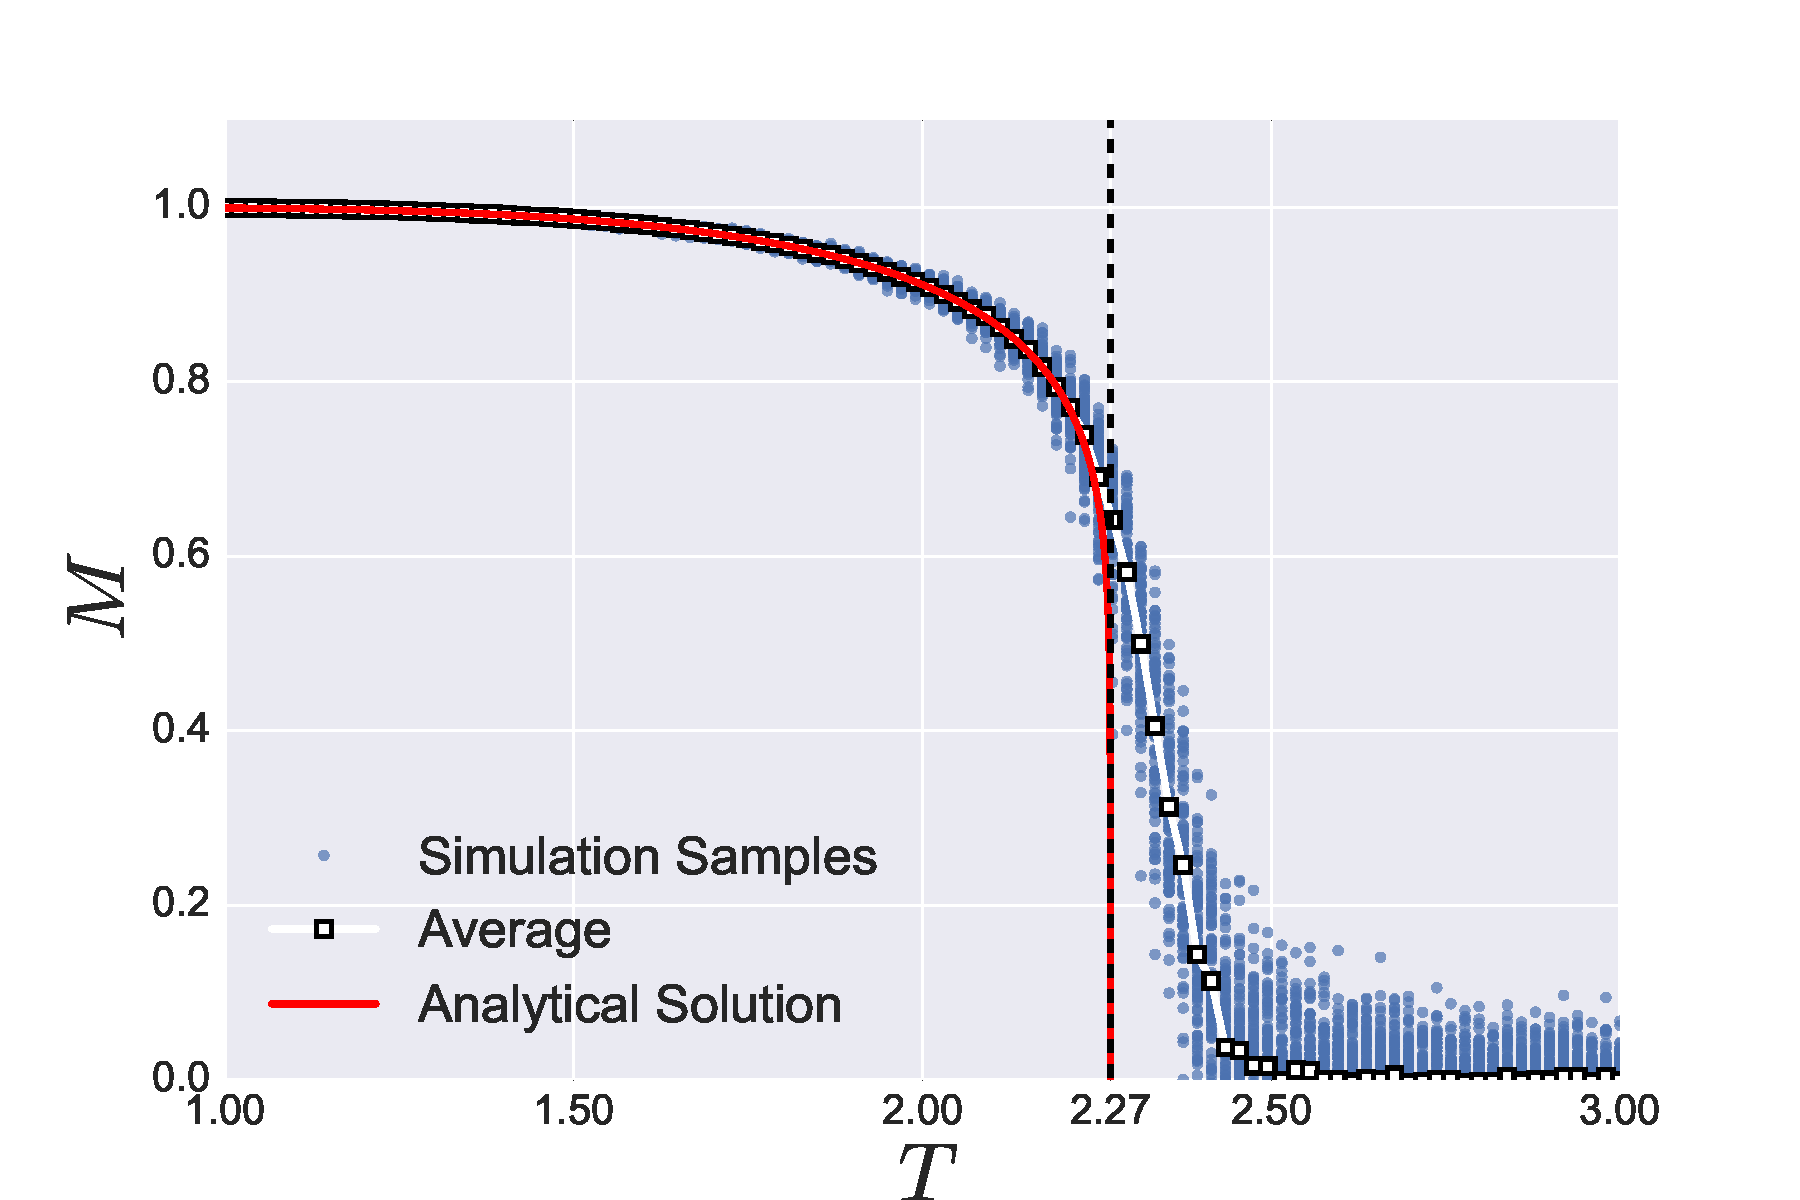
\includegraphics[width=0.7\textwidth]{chapters/ch2-crit/figs/ising_phase}
\end{center}
\caption{Spontaneous magnetization as a function of temperature for the Ising
    model. The simulations were performed in a $128\times128$ square lattice.
    As temperature rises, thermal fluctuations dominate the spin dynamics
    destroying the correlations. Above the critical temperature of
    $T_c=2/\log(1+\sqrt{2})\approx 2.269$ the value of $M$ should reach zero,
    although due to finite size effects we still observe some magnetization
    beyond this point. The red line shows the illustrious solution
    developed by Onsager~\cite{Onsager1944}, where
    $M={[1-{(\sinh{2/T})}^{-4}]}^{1/8}$.}
\label{fig:ising_phase}
\end{figure}

Let us take a look at the phase diagram of the Ising model.
Figure~\ref{fig:ising_phase2} shows the 2D square lattice version. We observe a
first order phase transition at $h=0$ and $T<T_c$, where the magnetization
discontinuously flips direction. At $T=T_c$ the transition becomes continuous.
The value of the critical point is given by
\begin{equation}
    T_{c}=
    \frac{2J}{k_{b}\log\left(1+\sqrt{2}\right)}
    \approx2.27\frac{J}{k_{b}},
\end{equation}
and the magnetization along the coexistence line is~\cite{Yang1952}
\begin{equation}
    \label{eq:ons}
    M={\left[1-\sinh^{-4}\left(\frac{2J}{k_{b}T}\right)\right]}^{1/8}.
\end{equation}
See Figure~\ref{fig:ising_phase} for the overall behavior of $M$.
From Eq.~\ref{eq:ons} we can determine that $\beta=1/8$. The values of the
other exponents of the Ising universality class can be seen in
Table~\ref{tab:univ}. The Ising universality class encompass more than just the
ferromagnetic transition. For instance, the liquid-vapor critical point (like
the one found in the water phase diagram) also falls in the same class. To this
day no exact solution for three dimensions have been presented, as it happens
with most higher dimension models.

%From a computational perspective, simulating the Ising model is particularly
%simple using the Metropolis-Hastings algorithm~\cite{Hastings1970}. At each
%step chose a random spin of the lattice and compute the change in energy
%$\Delta E$ that would occur if you were to flip the spin. In a square lattice
%this is given by (assuming $h=0$ and $J/k_b=1$)
%\begin{equation}
    %\Delta E=2s\left(i,j\right)\left[s\left(i+1,j\right)+
    %s\left(i-1,j\right)+s\left(i,j+1\right)+s\left(i,j-1\right)\right],
%\end{equation}
%where $s(i,j)$ is the spin at position $x=ai$ and $y=aj$ and $a$ is the
%lattice constant. You actually perform the flip $s(i,j)\rightarrow -s(i,j)$ if
%$\Delta E\leq 0$. If not, you should still perform the flip randomly with
%probability $\exp(-\Delta E / T)$. Thermodynamical properties can be computed from
%the fluctuation-dissipation theorem~\cite{Nishimori2011}, that 
%\begin{equation}
    %c=\frac{\left\langle E^{2}\right\rangle -\left\langle E\right\rangle ^{2}}{T^2},
    %\,\,\,\,\,\,\,\,
    %\chi=\frac{\left\langle M^{2}\right\rangle -\left\langle M\right\rangle ^{2}}{T}
%\end{equation}
%Figure~\ref{fig:ising_phase} shows the magnetization as a function of
%temperature compared to Onsager's solution, and Figure~\ref{fig:ising_cx} shows the
%specific heat and susceptibility, along with their characteristic divergence
%near the theoretical critical point.

%\begin{figure}
%\begin{center}
    %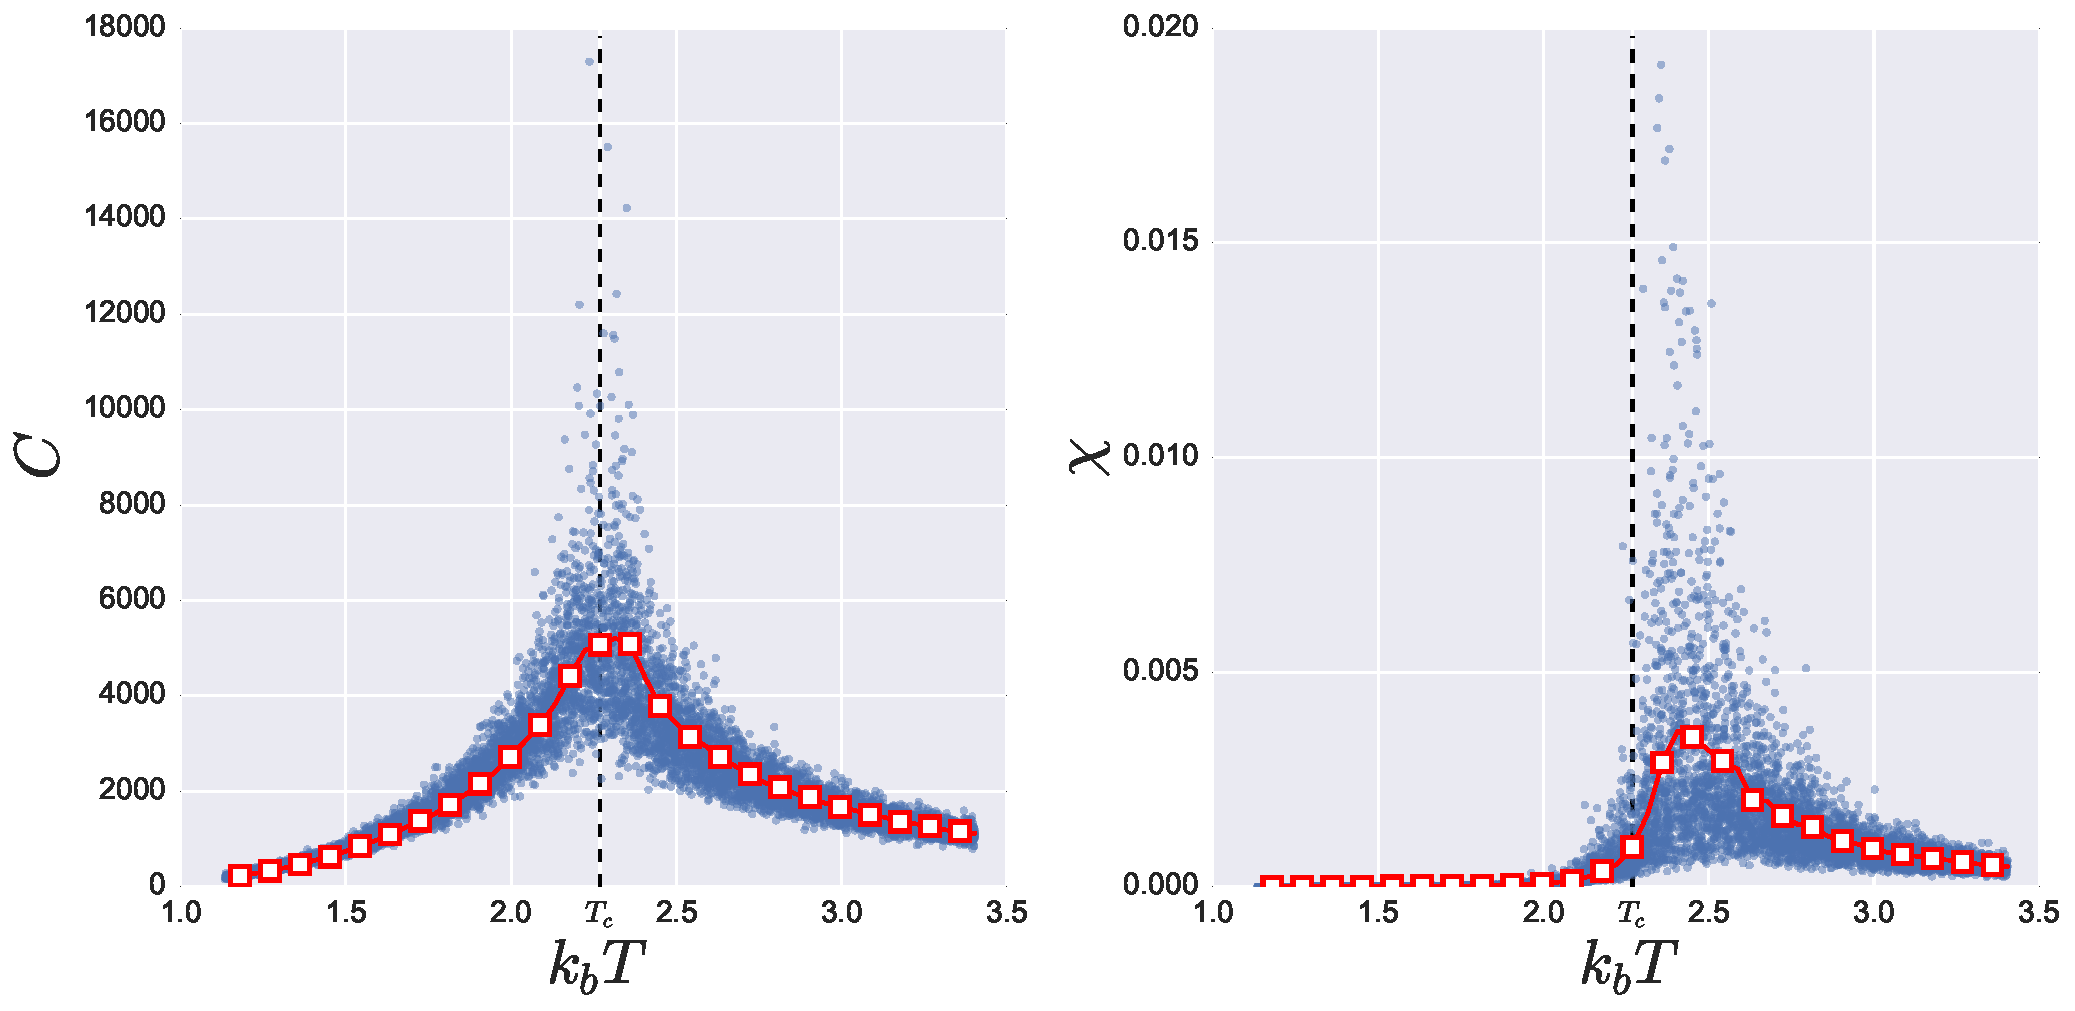
\includegraphics[width=\textwidth]{chapters/ch2-crit/figs/ising_cx}
%\end{center}
%\caption{Specific heat and susceptibility computed from a simulation of the
    %Ising model in a $64\times 64$ square lattice. They are computed from the
    %fluctuation-dissipation theorem, where $c=T^{-2}\left(\left\langle
    %E^{2}\right\rangle -\left\langle E\right\rangle ^{2}\right)$ and
    %$\chi=T^{-1}\left(\left\langle M^{2}\right\rangle -\left\langle
    %M\right\rangle ^{2}\right)$. Both quantities show the characteristic
    %diverging behavior near the critical point at $T_c\approx 2.27$.}
%\label{fig:ising_cx}
%\end{figure}



\subsection{Percolation}
\label{sec:perc}

\begin{figure}[b]
\begin{center}
    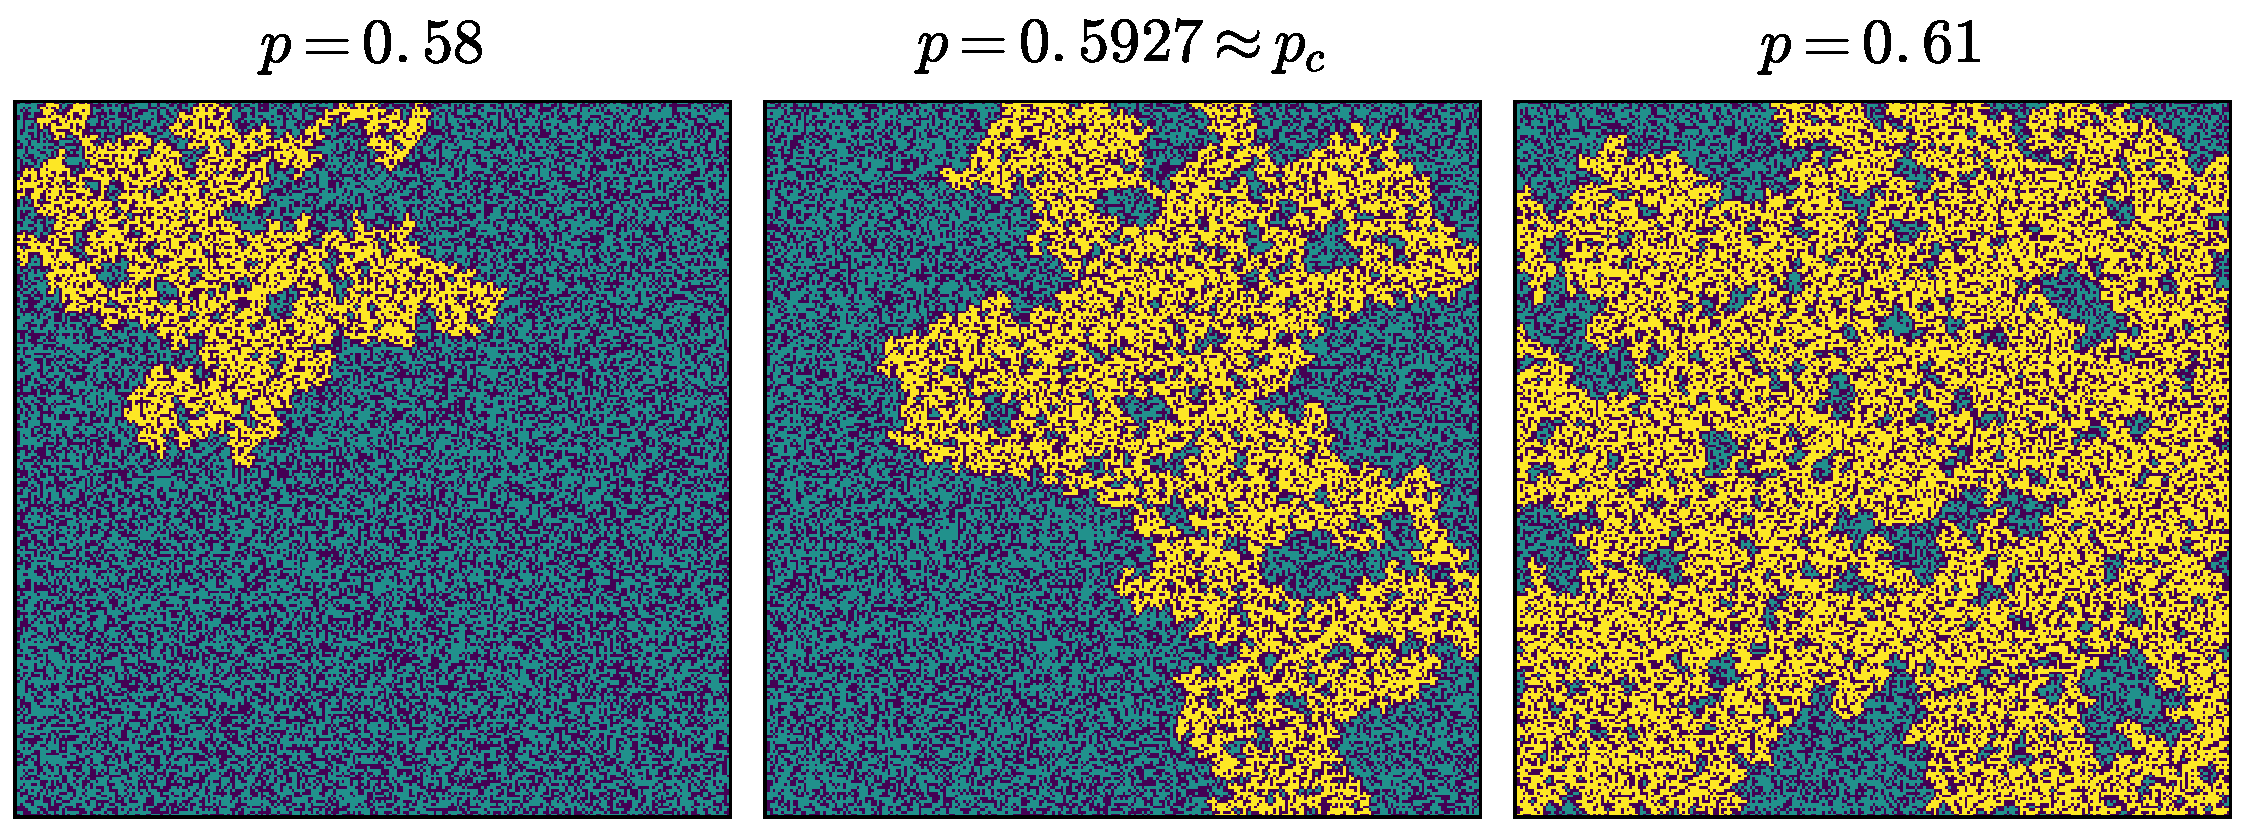
\includegraphics[width=0.9\textwidth]{chapters/ch2-crit/figs/isoperco}
\end{center}
%\caption{Realizations of the percolation model in a square lattice with three
    %different occupation probabilities $p$. Black sites are unoccupied, blue
    %ones are occupied, and the largest cluster is painted yellow. For small
    %values of $p$, there is no cluster that connects opposite sides of the
    %systems. Above the critical point however, the largest cluster promotes a
    %global connectivity.}
\caption{Percolation model with three
    different occupation probabilities $p$. Black sites are unoccupied, blue
    ones are occupied, and the largest cluster is painted yellow. 
    We only observe a spanning cluster connecting different sides of the system
    when $p\geq p_c$.}
\label{fig:isoperco}
\end{figure}

While fiercely competing with the Ising model in terms of popularity,
percolation certainly wins in terms of simplicity. Introduced in 1957 by
Broadbent and Hammersley~\cite{Broadbent1957}, the question they were trying to
answer was very humble: say we block a water pipe with a rock, how porous
should the rock be for the water to be able to flow, even if at a very low
rate? To find an answer, they modeled the rock as a square lattice where each
site can be either occupied by the rocky substrate or a hole. The measure of
the porosity is the ratio between the number of holes and the total number of
sites in the lattice. Of course, the more porous is a rock, the more holes it
has. Assuming these holes are randomly and uniformly distributed on the
substrate, they will often, by pure chance, fall into clusters of neighboring
holes, which are in fact just bigger holes. Water will be able to flow through
the rock only if we have a cluster that traverse the system from one side to
the other. This cluster is called the \textit{percolating} (or spanning)
cluster. So we can reframe the initial question as follows: whats the smallest
value of porosity where a percolating cluster will always be present in the
system. A 0\% porous rock would obviously always be impermeable, and a 100\%
porous rock is just no rock at all. But how about 50\%, or 40\%, or 60\%? The
answer naturally depends on the size of the lattice, but for a very large one
we observe the existence of a critical porosity $p_c$ below which we never
observe a percolating cluster, while above $p_c$ one is away present. See
Figure~\ref{fig:isoperco} for some realizations of the percolation process in
two dimensions in each state: subcritical, critical and supercritical.

\begin{figure}[h]
\begin{center}
    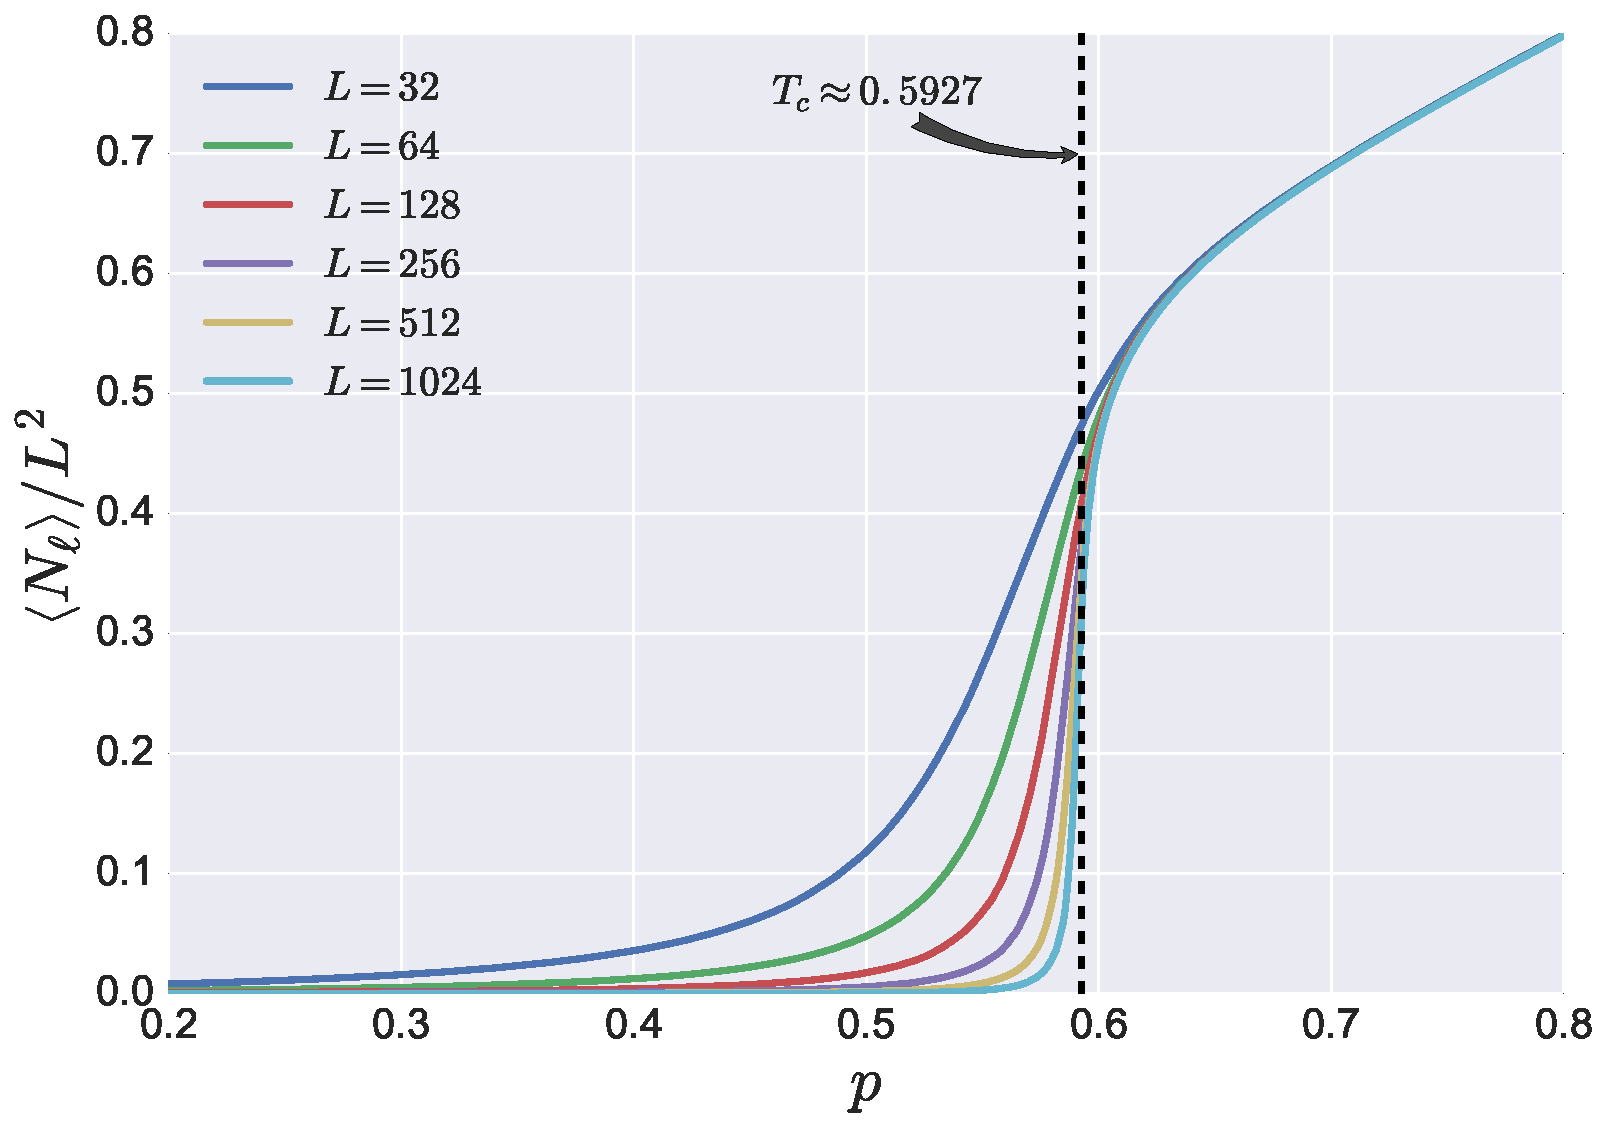
\includegraphics[width=0.7\textwidth]{chapters/ch2-crit/figs/isoperco2}
\end{center}
\caption{The order parameter of the percolation model as a function of the
    occupation probability for various system sizes. The order parameter here
    is defined as the fraction of the system occupied by the largest cluster.
    In the thermodynamical limit, the largest cluster have a finite size for
    $T<T_c\approx 0.592746$, that is, it occupies a negligible fraction of the
    system. Above the critical point the largest cluster is infinite and occupies
    a finite fraction.}
\label{fig:isoperco2}
\end{figure}

This is the core of percolation theory, initially motivated by a transport
problem. From a more generic perspective, Stauffer summarizes it
better~\cite{Stauffer1994}: ``Each site of a lattice is occupied randomly with
probability $p$ independent of its neighbors. Percolation theory deals with the
clusters of neighboring occupied sites thus formed''. At this point it is clear
the system goes through a phase transition, each phase defined by the presence
or not of a spanning cluster, which promotes a global connectivity of the
system. We can study its properties by defining an order parameter $P$ as the
fraction of the system occupied by the largest cluster, that is $P=N_\ell/N$
($N$ being the number of sites in the lattice and $N_\ell$ the number of sites
belonging to the largest cluster). For small values of $p$, the largest cluster
occupies a finite area of the system, which is basically a null fraction for a
large enough system. As $p$ approaches a critical probability $p_c$, the
largest cluster grows to the order of the system size.
Figure~\ref{fig:isoperco2} shows how the order parameter behaves for various
sizes of a square lattice. It shows that as the system reaches the
thermodynamical limit, the order parameter closely resembles as a second order
phase transition.

The type of percolation described so far, where we occupy the sites of a lattice
is called \textit{site percolation}. Alternatively we could instead occupy the
bonds. It is as if we had an empty isolating substrate with a potential
difference $V$ put along it. We then randomly insert resistors between the
sites with probability $p$. The system will have percolated when it has a
bridge of resistors traversing it, along which electrical current can flow,
thus passing from an isolating phase to a conductive one~\cite{Kirkpatrick1973}.
Figure~\ref{fig:sitebond} illustrate the difference between site and bond
percolation.

\begin{figure}[b]
\begin{center}
    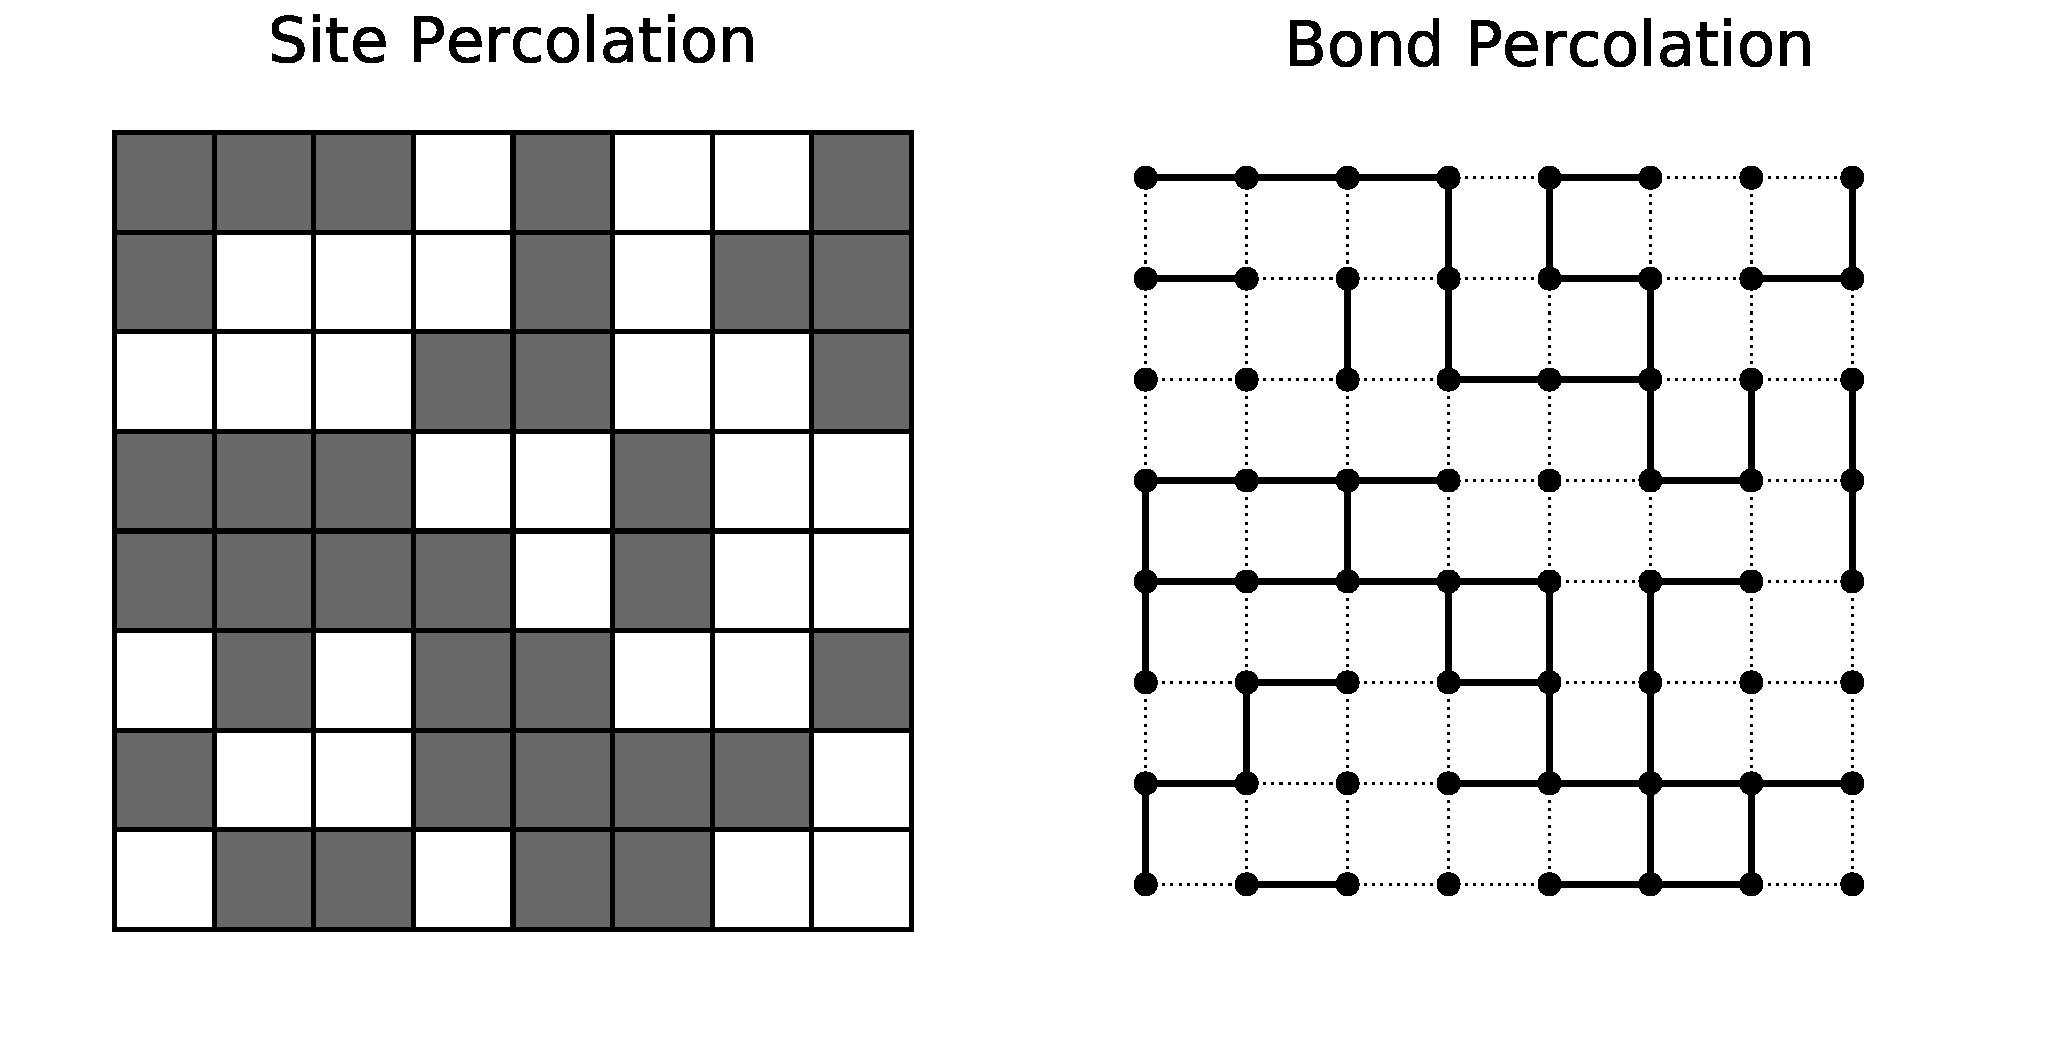
\includegraphics[width=0.8\textwidth]{chapters/ch2-crit/figs/sitebond}
\end{center}
\caption{Examples of site and bond percolation in a square lattice.
    In site percolation each site is occupied with probability $p$, while
    in bond percolation any two neighboring sites are connected with a bond
    with probability $p$.}
\label{fig:sitebond}
\end{figure}

The exact value of the critical point is non universal and depends on whether
it is site or bond percolation and on the lattice choice. The two more notorious
examples are site percolation on a square lattice, that has a critical point at
$p_c\approx0.592746$ and site percolation on a triangular lattice at $p_c=0.5$.
Values of the critical point for various other lattices are shown in
Table~\ref{tab:perc}.

The critical behavior of the percolation model is usually given by two critical
exponents. The first is the \textit{Fisher exponent} $\tau$, related to
the distribution of the cluster sizes at criticality
\begin{equation}
    \label{eq:ns1}
    n_s\sim s^{-\tau},\;\;\;\;\;\;p=p_c,
\end{equation}
where $s$ is the size of a cluster and $n_s$ is the number of clusters with
size $s$ in the system. Below the critical point, the distribution has an
exponential cutoff
\begin{equation}
    \label{eq:ns2}
    n_s\sim s^{-\tau}e^{-cs},\;\;\;\;\;\;p<p_c,
\end{equation}
where we define the other important critical exponent $\sigma$, related
to the scaling of the cutoff parameter $c$
\begin{equation}
    \label{eq:sig}
    c\sim \left|p-p_c\right|^{-1/\sigma}.
\end{equation}
From these two exponents, $\tau$ and $\sigma$, we can determine all others
listed in Section~\ref{sec:universality}. For instance take the order parameter
as defined before. From Section~\ref{sec:universality} we know it scales as
\begin{equation}
    P\sim\left|p-p_c\right|^{-\beta}.
\end{equation}
\begin{table}
\newcolumntype{L}[1]{>{\raggedright\let\newline\\\arraybackslash\hspace{0pt}}m{#1}}
\begin{centering}
\begin{tabular}{lll}
\bottomrule[0.1mm]
\toprule[0.1mm]
\textbf{Lattice} & \textbf{Site} & \textbf{Bond}     \\
\toprule[0.1mm]
Square           & 0.592746      & 0.5      \\[0.2cm]
Triangular       & 0.5           & 0.5      \\[0.2cm]
Honeycomb        & 0.6962        & 0.65271  \\[0.2cm]
Diamond          & 0.6962        & 0.65271  \\[0.2cm]
Simple Cubic     & 0.3116        & 0.2488   \\[0.2cm]
BCC              & 0.246         & 0.1803   \\[0.2cm]
FCC              & 0.198         & 0.119    \\[0.2cm]
\toprule[0.1mm]
\toprule[0.1mm]
\end{tabular}
\par\end{centering}
\caption{Percolation threshold for site and bond percolation in several 2D and
    3D regular lattices. Reproduced from~\cite{Stauffer1994}.}
\label{tab:perc}
\end{table}

We defined $P$ as the expected size of the largest cluster, which
we can assume should be distributed like $n_s(p_c)-n_s(p)$ for
$p < p_c$. Therefore, using Eqs.~\ref{eq:ns1} and~\ref{eq:ns2}
\begin{eqnarray}
    P & \sim & \int\left[n_{s}\left(p_{c}\right)-n_{s}\left(p\right)\right]sds\\
      & \sim & \int s^{1-\tau}\left[1-e^{-cs}\right]ds
\end{eqnarray}
Integrating by parts and making the transformation $s\rightarrow z/c$ yields
\begin{eqnarray}
P & \sim & c^{\tau-2}\int z^{2-\tau}e^{-z}dz\\
 & \propto & c^{\tau-2}\\
 & \propto & \left|p-p_{c}\right|^{\left(\tau-2\right)/\sigma}
\end{eqnarray}
which gives us the relation for $\beta$ as a function of $\tau$ and $\sigma$
\begin{equation}
    \beta=\frac{\tau-2}{\sigma}.
\end{equation}
    
In a similar way, we can find $\gamma$ by using the susceptibility, defined in
the percolation context as the second moment of the cluster size distribution
\begin{eqnarray}
    \chi & = & \int s^{2}n_{s}ds\\
      & = & \int s^{2-\tau}e^{-cs}ds\\
      & = & c^{\tau-3}\int z^{2-\tau}e^{-z}dz
    \label{eq:susperco}
\end{eqnarray}
Since the integral term in Eq.~\ref{eq:susperco} is a constant, we have
\begin{eqnarray}
    \chi & \propto & c^{\tau-3}\\
 & \propto & \left|p-p_{c}\right|^{-\left(3-\tau\right)/\sigma}.
\end{eqnarray}
which leads, following the relation of the $\gamma$ exponent
\begin{equation}
    \gamma=\frac{3-\tau}{\sigma}
\end{equation}


Once $\beta$ and $\gamma$ have been determined as a function of $\tau$ and
$\sigma$, all other critical exponents can be derived using the scaling
and hyperscaling relations (Eqs.~\ref{eq:scal1}--\ref{eq:scal2},~\ref{eq:hs1},
and~\ref{eq:hs2}). Here
are all of the others
\begin{eqnarray}
    \alpha & = & 1-\frac{\tau-1}{\sigma}\\
    \delta & = & \frac{1}{\tau-2}\\
    \nu    & = & \frac{\tau-1}{\sigma d}\\
    \eta   & = & 2-d\frac{3-\tau}{\tau-1}
\end{eqnarray}

From a numerical standpoint, percolation does not pose too much problem, as
there are many algorithms around that allow for the simulation of very large
lattices, basically limited only by the memory of the
computer~\cite{Newman2000}.

The critical exponents of two dimensional site percolation lattice have been
exactly computed in the triangular lattice using Schramm Loewner
Evolutions~\cite{Smirnov2001} (we will get there in Chapter~\ref{ch:sle}). The
values found are $\tau=187/91$ and $\sigma=36/91$. The other exponents can be
found in Table~\ref{tab:univ}. Other lattices have not been solved neither
proved to be in the same universality class, although the numerical evidence
that this is the fact is overwhelming.

Despite the initial motivation coming from transport theory, the percolation
model is much more general than that, being applied to various other areas like
the study of gelation of polymers~\cite{DeCandia2005}, conductivity in
semiconductors~\cite{Ambegaokar1971}, and the dynamics of the immune
system~\cite{Stewart1991}, among others~\cite{Sahimi1994}.

Just like the Ising model, the simplicity of percolation is ripe for the
development of derivative models, aiming to elucidate other aspects of phase
transitions. These include cooperative sequential adsorption~\cite{Araujo2013},
explosive percolation~\cite{Achlioptas2009} and invasive
percolation~\cite{Wilkinson1983}, to name just a few.


